%% abtex2-modelo-trabalho-academico.tex, v-1.9.6

\documentclass[
	12pt,				% tamanho da fonte
	openright,			% capítulos começam em pág ímpar (insere página vazia caso preciso)
	oneside,			% para impressão em recto e verso (twoside). Oposto a (oneside)
	a4paper,			% tamanho do papel. 
	chapter=TITLE,		% títulos de capítulos convertidos em letras maiúsculas
	section=TITLE,		% títulos de seções convertidos em letras maiúsculas
	sumario=abnt-6027-2012,
	english,			% idioma adicional para hifenização
	brazil,				% o último idioma é o principal do documento
	fleqn,				% equações alinhadas a esquerda
	]{abntex2}

% ----------------------------------------------------------
% Pacotes básicos 
% ----------------------------------------------------------
\usepackage{nccmath}
\usepackage{amsmath}							% Pacote matemático
\usepackage{amssymb}							% Pacote matemático
\usepackage{amsfonts}							% Pacote matemático
%\usepackage{lmodern}							% Usa a fonte Latin Modern		
\usepackage{mathptmx} 							% Usa a fonte Times New Roman
\usepackage[T1]{fontenc}						% Selecao de codigos de fonte.
\usepackage[utf8]{inputenc}						% Codificacao do documento (conversão automática dos acentos)
\usepackage{lastpage}							% Usado pela Ficha catalográfica
\usepackage{indentfirst}						% Indenta o primeiro parágrafo de cada seção.
\usepackage[dvipsnames,table]{xcolor}			% Controle das cores
\usepackage{graphicx}							% Inclusão de gráficos
\usepackage{microtype} 							% para melhorias de justificação
\usepackage{lipsum}								% para geração de dummy text
\usepackage[brazilian,hyperpageref]{backref}	% Paginas com as citações na bibl
\usepackage[alf,abnt-emphasize=bf,abnt-full-initials=yes]{abntex2cite}					% Citações padrão ABNT
%\usepackage[num]{abntex2cite}					% Citações padrão ABNT numérica
\usepackage{adjustbox}							% Pacote de ajuste de boxes
\usepackage{subcaption}							% Inclusão de Subfiguras e sublegendas		
\usepackage{enumitem}							% Personalização de listas
\usepackage{siunitx}							% Grandezas e unidades
\usepackage[section]{placeins}					% Manter as figuras delimitadas na respectiva seção com a opção [section]
\usepackage{multirow}							% Multi colunas nas tabelas
\usepackage{array,tabularx} 					% Pacotes de tabelas
\usepackage{booktabs}							% Pacote de tabela profissonal
\usepackage{rotating}							% Rotacionar figuras e tabelas
\usepackage{xfrac}								% Fazer frações n/d em linha
\usepackage{bm}									% Negrito em modo matemático
\usepackage{xstring}							% Manipulação de strings
\usepackage{pgfplots}							% Pacote de Gráficos
\usepackage{tikz}								% Pacote de Figuras
\usepackage[american, cuteinductors,smartlabels, fulldiode, siunitx, americanvoltages, oldvoltagedirection, smartlabels]{circuitikz}	% Pacote de circuitos elétricos
\usepackage{chemformula}						% Pacote para fórmulas químicas
\usepackage{chngcntr}							% Pacote usado para deixar numeração de equações sequencial
\counterwithout{equation}{chapter}
% fonte: https://latex.org/forum/viewtopic.php?t=15392

% Comando para deixar numeração das equações contínua (1), (2), (3)... ao invés de organizar por capítulos (1.1)(1.2)... (2.1)(2.2)
%\renewcommand{\theequation}{\arabic{equation}}

%\numberwithin{equation}{section}

% Cabecalho cabeçalho somente com numeração de página 10pt
\makepagestyle{PagNumReduzida}
\makeevenhead{PagNumReduzida}{\ABNTEXfontereduzida\thepage}{}{}
\makeoddhead{PagNumReduzida}{}{}{\ABNTEXfontereduzida\thepage}
%fonte: https://github.com/abntex/abntex2/wiki/HowToCustomizarCabecalhoRodape
%fonte: Manual memoir seção 7.3 pg. 111 pdf http://linorg.usp.br/CTAN/macros/latex/contrib/memoir/memman.pdf 

% Personalização das opções das listas
\setlist[itemize]{leftmargin=\parindent}

% Citação online --- MODIFICAR ---
\newcommand{\citeshort}[1]{\citeauthoronline{#1}~(\citeyear{#1})}

\newcommand{\me}[1]{Elaborado pelo autor (#1).}

% Configuração do pgfplots
\pgfplotsset{compat=newest} %compat=1.14
\pgfplotsset{plot coordinates/math parser=false} 
\newlength\figureheight 
\newlength\figurewidth 

% Libraries do TiKz
\usetikzlibrary{quotes,angles,arrows}
\usetikzlibrary{through,calc,math}
\usetikzlibrary{graphs,backgrounds,fit}
\usetikzlibrary{shapes,positioning,patterns,shadows}
\usetikzlibrary{decorations.pathreplacing}
\usetikzlibrary{shapes.geometric}
\usetikzlibrary{arrows.meta}
\usetikzlibrary{external}

%\tikzexternalize[]
%\tikzexternalenable
%\tikzexternalize
%\tikzexternaldisable
%\tikzset{external/force remake}
%\tikzexternalize[shell escape=-enable-write18]

% Configurações do CircuiTiKz
\ctikzset{bipoles/thickness=1}
%\ctikzset{bipoles/length=1.2cm}
\ctikzset{monopoles/ground/width/.initial=.2}
\ctikzset{bipoles/resistor/height=0.25}
\ctikzset{bipoles/resistor/width=0.6}
\ctikzset{bipoles/capacitor/height=0.5}
\ctikzset{bipoles/capacitor/width=0.15}
\ctikzset{bipoles/generic/height=0.25}
\ctikzset{bipoles/generic/width=0.6}
%\ctikzset{bipoles/capacitor polar/length=0.5}
%\ctikzset{bipoles/diode/height=.375}
%\ctikzset{bipoles/diode/width=.3}
%\ctikzset{tripoles/thyristor/height=.8}
%\ctikzset{tripoles/thyristor/width=1}
\ctikzset{bipoles/vsourcesin/height=.5}
\ctikzset{bipoles/vsourcesin/width=.5}
\ctikzset{bipoles/cvsourceam/height=.6}
\ctikzset{bipoles/cvsourceam/width=.6}
%\ctikzset{tripoles/european controlled voltage source/width=.4}

\tikzstyle{every node}=[font=\footnotesize]
\tikzstyle{every path}=[line width=0.25pt,line cap=round,line join=round]
%\tikzstyle{every path}=[line cap=round,line join=round]


% Definição de cores MATLAB
\definecolor{matlab_blue}{rgb}	{         0,    0.4470,    0.7410}
\definecolor{matlab_orange}{rgb}{    0.8500,    0.3250,    0.0980}
\definecolor{matlab_yellow}{rgb}{    0.9290,    0.6940,    0.1250}
\definecolor{matlab_violet}{rgb}{    0.4940,    0.1840,    0.5560}
\definecolor{matlab_green}{rgb}	{	 0.4660,    0.6740,    0.1880}
\definecolor{matlab_lblue}{rgb}	{    0.3010,    0.7450,    0.9330}
\definecolor{matlab_red}{rgb}	{    0.6350,    0.0780,    0.1840}

% Personalização das legendas
\usepackage[format = plain, %hang
			justification = centering,
			labelsep = endash,
			singlelinecheck = false,
			skip = 6pt,
			listformat = simple,
			font = footnotesize]{caption}	

% Personalização das unidades
\sisetup{output-decimal-marker = {,}}
\sisetup{exponent-product = \cdot} % , output-product = \cdot}
\sisetup{tight-spacing=true}
\sisetup{group-digits = false}

% Personalizações de tipo de colunas de tabelas
\newcolumntype{L}[1]{>{\raggedright\let\newline\\\arraybackslash\hspace{0pt}}m{#1}}
\newcolumntype{C}[1]{>{\centering\let\newline\\\arraybackslash\hspace{0pt}}m{#1}}
\newcolumntype{R}[1]{>{\raggedleft\let\newline\\\arraybackslash\hspace{0pt}}m{#1}}

% Personalizações de cores da UDESC
\definecolor{CapaAmareloUDESC}{RGB}{243,186,83}		% Especializacao
\definecolor{CapaVerdeUDESC}{RGB}{0,112,52}			% Mestrado
\definecolor{CapaVermelhoUDESC}{RGB}{171,35,21}		% Doutorado
\definecolor{CapaAzulUDESC}{RGB}{38,54,118} 		% Pós-Doutorado

% CONFIGURAÇÕES DE PACOTES
% Configurações do pacote backref
% Usado sem a opção hyperpageref de backref
\renewcommand{\backrefpagesname}{Citado na(s) página(s):~}
% Texto padrão antes do número das páginas
\renewcommand{\backref}{}
% Define os textos da citação
\renewcommand*{\backrefalt}[4]{
	\ifcase #1 %
	Nenhuma citação no texto.%
	\or
	Citado na página #2.%
	\else
	Citado #1 vezes nas páginas #2.%
	\fi}%

% alterando o aspecto da cor azul
%\definecolor{blue}{RGB}{41,5,195}

% informações do PDF
\makeatletter
\hypersetup{
	%pagebackref=true,
	pdftitle={\@title}, 
	pdfauthor={\@author},
	pdfsubject={\imprimirpreambulo},
	pdfcreator={LaTeX with abnTeX2},
	pdfkeywords={abnt}{latex}{abntex}{abntex2}{trabalho academico}, 
	colorlinks=true,       		% false: boxed links; true: colored links
	linkcolor=black,          	% color of internal links
	citecolor=black,        	% color of links to bibliography
	filecolor=black,      		% color of file links
	urlcolor=black,
	bookmarksdepth=4
}
\makeatother


\makeatletter
\newcommand{\includetikz}[1]{%
	\tikzsetnextfilename{#1}%
	\input{#1.tex}%
}
\makeatother

% ---
% Possibilita criação de Quadros e Lista de quadros.
% Ver https://github.com/abntex/abntex2/issues/176
%
\newcommand{\quadroname}{Quadro}
\newcommand{\listofquadrosname}{Lista de quadros}

\newfloat[chapter]{quadro}{loq}{\quadroname}
\newlistof{listofquadros}{loq}{\listofquadrosname}
\newlistentry{quadro}{loq}{0}

% configurações para atender às regras da ABNT
\setfloatadjustment{quadro}{\centering}
\counterwithout{quadro}{chapter}
\renewcommand{\cftquadroname}{\quadroname\space} 
\renewcommand*{\cftquadroaftersnum}{\hfill--\hfill}

\setfloatlocations{quadro}{hbtp} % Ver https://github.com/abntex/abntex2/issues/176
% ---


% Espaçamento depois do título
\setlength{\afterchapskip}{0.7\baselineskip}
% O tamanho do parágrafo é dado por:
\setlength{\parindent}{1.25cm}
% Controle do espaçamento entre um parágrafo e outro:
\setlength{\parskip}{0.0cm}  % tente também \onelineskip
%\SingleSpacing % Espaçamento simples 
\OnehalfSpacing % Espaçamento 1,5
%\DoubleSpacing	% Espaçamento duplo

% ---
% Margens - NBR 14724/2011 - 5.1 Formato
% ---
\setlrmarginsandblock{3cm}{2cm}{*}
\setulmarginsandblock{3cm}{2cm}{*}
\checkandfixthelayout[fixed]
% ---


% To use externalize consider
%https://tex.stackexchange.com/questions/182783/tikzexternalize-not-compatible-with-miktex-2-9-abntex2-package
%Lauro Cesar digged into the problem until he came with a solution for me to test. And it Works!
%
%According to this link:
%
%The package calc changed the commands \setcounter and friends to be fragile. So you have to make them robust. The example below uses etoolbox with \robustify:
%
\usepackage{etoolbox}
\robustify\setcounter
\robustify\addtocounter
\robustify\setlength
\robustify\addtolength


%% How to silence memoir class warning against the use of caption package?
%% https://tex.stackexchange.com/questions/391993/how-to-silence-memoir-class-warning-against-the-use-of-caption-package
%\usepackage{silence}
%\WarningFilter*{memoir}{You are using the caption package with the memoir class}
%\WarningFilter*{Class memoir Warning}{You are using the caption package with the memoir class}

% --------------------------------------------------------
% INICIO DAS CUSTOMIZACOES PARA A UDESC
% --------------------------------------------------------

% --------------------------------------------------------
% Fontes padroes de part, chapter, section, subsection e subsubsection
% --------------------------------------------------------
% --- Chapter ---
\renewcommand{\ABNTEXchapterfont}{\fontseries{b}} %\bfseries
\renewcommand{\ABNTEXchapterfontsize}{\normalsize}
% --- Part ---
\renewcommand{\ABNTEXpartfont}{\ABNTEXchapterfont}
\renewcommand{\ABNTEXpartfontsize}{\LARGE}
% --- Section ---
\renewcommand{\ABNTEXsectionfont}{\normalfont}
\renewcommand{\ABNTEXsectionfontsize}{\normalsize}
% --- SubSection ---
\renewcommand{\ABNTEXsubsectionfont}{\fontseries{b}} %\bfseries
\renewcommand{\ABNTEXsubsectionfontsize}{\normalsize}
% --- SubSubSection ---
\renewcommand{\ABNTEXsubsubsectionfont}{\itshape}
\renewcommand{\ABNTEXsubsubsectionfontsize}{\normalsize}

\renewcommand{\ABNTEXsubsubsubsectionfont}{\normalfont}
\renewcommand{\ABNTEXsubsubsubsectionfontsize}{\normalsize}
% ---

% --------------------------------------------------------
% Fontes das entradas do sumario
% --------------------------------------------------------

\renewcommand{\cftpartfont}{\ABNTEXpartfont\selectfont}
\renewcommand{\cftpartpagefont}{\normalsize\selectfont}

\renewcommand{\cftchapterfont}{\ABNTEXchapterfont\selectfont}
\renewcommand{\cftchapterpagefont}{\normalsize\selectfont}

\renewcommand{\cftsectionfont}{\ABNTEXsectionfont\selectfont}
\renewcommand{\cftsectionpagefont}{\normalsize\selectfont}

\renewcommand{\cftsubsectionfont}{\ABNTEXsubsectionfont\selectfont}
\renewcommand{\cftsubsectionpagefont}{\normalsize\selectfont}

\renewcommand{\cftsubsubsectionfont}{\normalfont\itshape\selectfont}
\renewcommand{\cftsubsubsectionpagefont}{\normalsize\selectfont}

\renewcommand{\cftparagraphfont}{\normalfont\selectfont}
\renewcommand{\cftparagraphpagefont}{\normalsize\selectfont}

% --------------------------------------------------------
% Usando os pacotes hyperref, uppercase... 
% Para deixar a section do toc uppercase precisa de:
% --------------------------------------------------------
\usepackage{textcase}

\makeatletter

\let\oldcontentsline\contentsline
\def\contentsline#1#2{%
	\expandafter\ifx\csname l@#1\endcsname\l@section
	\expandafter\@firstoftwo
	\else
	\expandafter\@secondoftwo
	\fi
	{%
		\oldcontentsline{#1}{\MakeTextUppercase{#2}}%
	}{%
		\oldcontentsline{#1}{#2}%
	}%
}
\makeatother

% --------------------------------------------------------
% Renomenando as entradas de APÊNDICES E ANEXOS
% --------------------------------------------------------

\renewcommand{\apendicesname}{AP\^ENDICES}
\renewcommand{\anexosname}{ANEXOS}


% Manipulação de Strings
%\RequirePackage{xstring}

% Comando para inverter sobrenome e nome
\newcommand{\invertname}[1]{%
	\StrBehind{#1}{{}}, \StrBefore{#1}{{}}%
}%


% --------------------------------------------------------
% Alterando os estilos de Caption e Fonte
% --------------------------------------------------------
\makeatletter
% Define o comando \fonte que respeita as configurações de caption do memoir ou do caption
\renewcommand{\fonte}[2][\fontename]{%
	\M@gettitle{#2}%
	\memlegendinfo{#2}%
	\par
	\begingroup
	\@parboxrestore
	\if@minipage
	\@setminipage
	\fi
	\ABNTEXfontereduzida
	\configureseparator
	\captiondelim{\ABNTEXcaptionfontedelim}
	\@makecaption{#1}{\ignorespaces #2}\par
	\endgroup}


\captionstyle[\raggedright]{\raggedright}

\makeatother

\setlength{\cftbeforechapterskip}{0pt plus 0pt}
\renewcommand*{\insertchapterspace}{}

\newlength{\mylen}	% New length to use with spacing
\setlength{\mylen}{1pt}

\setlength{\cftbeforechapterskip}{\mylen}
\setlength{\cftbeforesectionskip}{\mylen}
\setlength{\cftbeforesubsectionskip}{\mylen}
\setlength{\cftbeforesubsubsectionskip}{\mylen}
\setlength{\cftbeforesubsubsubsectionskip}{\mylen}


% ---
% Ajuste das listas de abreviaturas e siglas ; e símbolos [Personalizada para UDESC com espaçamento 1,5]
% ---

% ---
% Redefinição da Lista de abreviaturas e siglas [Personalizada para UDESC com espaçamento 1,5]
\renewenvironment{siglas}{%
	\pretextualchapter{\listadesiglasname}
	\begin{symbols} 
		\setlength{\itemsep}{0pt}	% Ajuste para Espaçamento 1,5
	}{% 
	\end{symbols}
	\cleardoublepage
}
% ---

% ---
% Redefinição da Lista de símbolos [Personalizada para UDESC com espaçamento 1,5]
\renewenvironment{simbolos}{%
	\pretextualchapter{\listadesimbolosname}
	\begin{symbols}
		\setlength{\itemsep}{0pt}	% Ajuste para Espaçamento 1,5
	}{%
	\end{symbols}
	\cleardoublepage
}
% ---	% inclui pacotes básicos 


% informações de dados para CAPA e FOLHA DE ROSTO

% título
\titulo{\textit{Text Mining} nas atas do Copom para criação de um índice de sentimento e averiguação de causalidade com variáveis macroeconômicas}%

\autor{Cairê {}Britto Barletta}%
\orientador{Prof.ª Dr.ª Marianne {}Zwilling Stampe}%

% o símbolo {} indica o sobrenome para a ficha catalográfica.

\instituicao{Universidade do Estado de Santa Catarina, Centro de Ciências da Administração e Socioeconômicas, Programa de Graduação em Ciências Econômicas}%

\tipotrabalho{Monografia (Graduação)}

\preambulo{Trabalho de Conclusão de Curso apresentado ao curso de Ciências Econômicas, do Centro de Ciências da Administração e Socioeconômicas, da Universidade do Estado de Santa Catarina, como requisito parcial para a obtenção do grau de Bacharel em Ciências Econômicas.}

\local{Florianópolis}%

\data{\the\year}%

% compila o indice
\makeindex


% início do documento

\begin{document}

\selectlanguage{brazil}
\frenchspacing  % retira espaço extra obsoleto entre as frases.


% ELEMENTOS PRÉ-TEXTUAIS

\pretextual

% capa

\renewcommand{\imprimircapa}{%
	\begin{capa}%
		\center

		{\fontseries{b}\selectfont\MakeTextUppercase{UNIVERSIDADE DO ESTADO DE SANTA CATARINA -- UDESC}}
		
		{\fontseries{b}\selectfont\MakeTextUppercase{Centro de Ciências da Administração e Socioeconômicas – ESAG}}
		
		{\fontseries{b}\selectfont\MakeTextUppercase{Departamento de Ciências Econômicas - DCE}}
		
		\vfill
		
		{\fontseries{b}\selectfont\MakeTextUppercase{\normalsize\imprimirautor}}
		
		\vfill
		\begin{center}
			{\fontseries{b}\selectfont\MakeTextUppercase{\imprimirtitulo}}
		\end{center}
		\vfill
		
		\vfill
		
		{\fontseries{b}\selectfont\MakeTextUppercase{\imprimirlocal}}
		\par
		{\fontseries{b}\selectfont \imprimirdata}
		\vspace*{1cm}
	\end{capa}
}

\imprimircapa					% Elemento Obrigatório
%folha de rosto

\makeatletter

\renewcommand{\folhaderostocontent}{
	\begin{center}
		
		{\fontseries{b}\selectfont\MakeTextUppercase{\imprimirautor}}
		
		\vfill
		
		\begin{center}
			{\fontseries{b}\selectfont\MakeTextUppercase{\imprimirtitulo}}
		\end{center}
	
		\vspace*{1.5cm}

		\abntex@ifnotempty{\imprimirpreambulo}{%
			\hspace{.45\textwidth}
			{\begin{minipage}{.5\textwidth}
					\SingleSpacing
					\imprimirpreambulo\par
					\vspace*{4pt}
					{\imprimirorientadorRotulo~\imprimirorientador\par}
					\abntex@ifnotempty{\imprimircoorientador}{%
						{\imprimircoorientadorRotulo~\imprimircoorientador}%
					}%
			\end{minipage}}%
		}%
	
		
		\vfill
		
	{\fontseries{b}\selectfont\MakeTextUppercase{\imprimirlocal}}
	\par
	{\fontseries{b}\selectfont \imprimirdata}
	\vspace*{1cm}
	\end{center}
}


% (o * indica que haverá a ficha bibliográfica)
% ---
\imprimirfolhaderosto*
% ---


	    	% Elemento Obrigatório

% Caso não utilize a Ficha Catalográfica entre na folha de rosto e retire o * de dentro do arquivo FolhadeRosto
%% inserir a ficha bibliografica

% para inserir a ficha catalográfica definitiva após a defesa do trabalho, recebida pela BU:

% \begin{fichacatalografica}
%     \includepdf{fig_ficha_catalografica.pdf}
% \end{fichacatalografica}


%	\setlength{\parindent}{0cm}
%	\setlength{\parskip}{0pt}
\begin{fichacatalografica}
	%\sffamily
	%\rmfamily
	\ttfamily \hbadness=10000
	\vspace*{\fill}					% posição vertical
	\begin{center}					% minipage centralizado
	Para gerar a ficha catalográfica de teses e \\ 
	dissertações acessar o link:  \\
	https://www.udesc.br/bu/manuais/ficha
	
	\vspace*{8pt}
	
%	\begin{minipage}[c]{8cm}
%	\centering \sffamily

%	\end{minipage}
	\fbox{\begin{minipage}[c]{12.5cm}	% largura
	\flushright
	{\begin{minipage}[c]{10.5cm}		% largura
	\vspace{1.25cm}
	%\footnotesize
	\setlength{\parindent}{1.5em}
	\noindent \invertname{\imprimirautor} \par
	\imprimirtitulo{ }/{ }\imprimirautor. -- \imprimirlocal, \imprimirdata .\par
	\pageref{LastPage} p. : il. ; 30 cm.\par
	\vspace{1.5em}
	\imprimirorientadorRotulo~\imprimirorientador.\par
	\imprimircoorientadorRotulo~\imprimircoorientador.\par
	\imprimirtipotrabalho~--~\imprimirinstituicao, \imprimirlocal, \imprimirdata.\par
	\vspace{1.5em}
		1. Palavra-chave.
		2. Palavra-chave.
		3. Palavra-chave.
 		4. Palavra-chave.
		5. Palavra-chave.
		I. \invertname{\imprimirorientador}.
		II. \invertname{\imprimircoorientador}.
		III. \imprimirinstituicao.
		IV. Título. %
	\vspace{1.25cm}	%		
	\end{minipage}%
	}% 
	\end{minipage}}%
	
	\vspace*{0.5cm}
	
	\end{center}
\end{fichacatalografica}	    % Elemento Obrigatório (Verso da Folha)
%% inserir errata

\begin{errata}
Elemento opcional. 

Exemplo:

\vspace{\onelineskip}

\begin{table}[htb]
\center
\begin{tabular}{|p{2.4cm}|p{2cm}|p{3cm}|p{3cm}|}
  \hline
   \textbf{Folha} & \textbf{Linha}  & \textbf{Onde se lê}  & \textbf{Leia-se}  \\
    \hline
    
   \hline
\end{tabular}
\end{table}

\end{errata}
% ---				    % Elemento Opcional
% inserir folha de aprovação

% pode-se utilizar este modelo até a aprovação do trabalho. Após isso, substituir todo o conteúdo deste arquivo por uma imagem da página assinada pela banca:

% \includepdf{folhadeaprovacao_final.pdf}

\begin{folhadeaprovacao}



	\begin{center}
		{\fontseries{b}\selectfont\MakeTextUppercase{\normalsize\imprimirautor}}
	\end{center}
    \vfill
    
	\vfill
	\begin{center}
		{\fontseries{b}\selectfont\MakeTextUppercase{\imprimirtitulo}}
	\end{center}
	\vfill

    
\abntex@ifnotempty{\imprimirpreambulo}{%
	\hspace{.45\textwidth}
	{\begin{minipage}{.5\textwidth}
			\SingleSpacing
			\imprimirpreambulo\par
			\vspace*{4pt}
			{\imprimirorientadorRotulo~\imprimirorientador\par}
			\abntex@ifnotempty{\imprimircoorientador}{%
				{\imprimircoorientadorRotulo~\imprimircoorientador}%
			}%
	\end{minipage}}%
}%


\vfill
        
	 \begin{center}
	 	
    	{\fontseries{b}\selectfont BANCA EXAMINADORA: }
    	\vspace*{1.75cm}
    
		Nome do Orientador e Titulação \par
		Nome da Instituição
	 \end{center}
	
    {Membros:} 
    
	\begin{center}
		\vspace*{1.25cm}
		Nome do Orientador e Titulação \par
		Nome da Instituição
		
		\vspace*{1.25cm}
		Nome do Orientador e Titulação \par
		Nome da Instituição
		
		\vspace*{1.25cm}
		Nome do Orientador e Titulação \par
		Nome da Instituição

	
	\end{center}
    
    \vspace*{\fill}  
    \begin{center}
    {\imprimirlocal, 05 de julho de \imprimirdata}
	\end{center}
    \vspace*{0.25cm}  
\end{folhadeaprovacao}		    % Elemento Obrigatório
% dedicatória

\begin{dedicatoria}
   \vspace*{\fill}
   \begin{flushright}
   \noindent
	Dedico este trabalho aos meus pais, \\
	sem vocês, eu nada seria.
   \end{flushright}

\end{dedicatoria}
% ---
			    % Elemento Opcional
% agradecimentos

\begin{agradecimentos}

Agradeço à minha família por ser o elemento de maior importância na minha vida. Em especial, à minha mãe Fabiane, ao meu pai Rodrigo, ao meu irmão Cainã, às minha avós Deuza e Rose, e aos meus avôs Antônio e Walter.

Agradeço à minha orientadora, Professora Doutora Marianne Zwilling Stampe, por todos os direcionamentos dados na elaboração do presente trabalho. Não só isso, agradeço pelos incentivos, comprometimento e parceria durante toda a jornada.

Agradeço também aos professores, mestres e doutores, que foram incondicionalmente importantes na minha trajetória, me marcando significativamente. Em especial, minha gratidão para Thais Waideman Niquito, Fernando Pozzobon, Marcello Beckert Zapelini, Marcos Vinicio Wink Junior, Analucia Vieira Fantin, Patrícia Bonini, Cassiano Ricardo Dalberto, e minha orientadora, Marianne Zwilling Stampe. Tenho imenso respeito e admiração pelo trabalho de todos vocês.

Agradeço também ao Fernando Zatt Schardosin, que me forneceu minha primeira e única bolsa de iniciação científica, logo no início da minha jornada acadêmica.

Agradeço aos amigos que já possuía antes de entrar na faculdade, por fazerem meus dias mais leves e agradáveis. Em especial, Peter Krause, Thales Zirbel, Yan Romano, Gabriel Lima, Rafael Aché, Pedro Aché e Arthur Masseli. Vocês são muito importantes para mim.

Agradeço às amizades que construí durante a graduação, por também fazerem meus dias mais leves e agradáveis, além de enfrentarem o percurso ao meu lado — na medida do possível. Em especial, Leonardo Oviedo, Bernardo Couto, José Marcelo Felleti, Isadora Zamprogna, Arthur Vier, Sabrina Bacaicoa, Nelson Ambros, Gabriel Akira, Henrique Matte e Arthur Rockenbach. A jornada não teria sido a mesma sem vocês.

Agradeço também pela oportunidade e experiência que o Clube de Finanças, projeto de extensão de liga acadêmica de mercado financeiro, me proporcionou.

Por fim, porém não menos importante, agradeço à Universidade do Estado de Santa Catarina e todos os colaboradores que nela trabalham.

Muito obrigado.

\end{agradecimentos}
		    % Elemento Opcional
%% epígrafe

\begin{epigrafe}
    \vspace*{\fill}
{
	\noindent\hspace{.5\textwidth}
	{\begin{minipage}{.5\textwidth}
		\begin{flushright}
			Escrever.
		\end{flushright}
	\end{minipage}}
	\vspace*{3cm}
}
\end{epigrafe}				% Elemento Opcional
% resumo em português

\setlength{\absparsep}{18pt} % ajusta o espaçamento dos parágrafos do resumo
\begin{resumo}

Este estudo apresenta a importância da comunicação e transparência de bancos centrais para a condução da política monetária. Dada esta relevância, foram empregadas técnicas de mineração textual e análise de sentimentos nas atas do Comitê de Política Monetária para criação de um índice, contemplando o período de 2006 até 2022. O índice foi então comparado com variáveis macroeconômicas, e após isso foram efetuados testes estatísticos, para contribuir com a robustez do  trabalho. Como resultados, aplicando Vetores Autorregressivos (VAR), através de Funções de Impulso-Resposta (IRF), pode-se dizer que dado um choque positivo no índice, a diferença da taxa básica de juros real é influenciada negativamente, enquanto que para a atividade econômica e para a produção industrial, percebe-se que a resposta é positiva com impactos descrescentes, onde todas se estabilizam em torno de zero no horizonte analisado, uma vez que os choques não possuem efeitos permanentes em séries estacionárias. 


 \textbf{Palavras-chave}: Mineração Textual. Análise de Sentimentos. Atas do Copom. Vetores Autorregressivos (VAR). Função Impulso-Resposta (IRF).
\end{resumo}
			    	% Elemento Obrigatório
% resumo em inglês
\begin{resumo}[Abstract]
 \begin{otherlanguage*}{english}

This research presents the importance around central banking communication and transparency to the conduction of monetary policy. Given this relevance, text mining and sentiment analysis techniques were applied to the Copom minutes in search of an index creation, covering the period from 2006 to 2022. The index was then compared with macroeconomic variables, and after that, statistical tests were performed to contribute to the robustness of the work. As a result, applying Autoregressive Vectors (VAR), through Impulse-Response Functions (IRF), it can be said that given a positive shock on the index, the real basic interest rate is negatively influenced, while for economic activity and for industrial production, it can be seen that the answer is positive, where they all stabilize around zero in the analyzed horizon, since the shocks do not have permanent effects in stationary series.

\textbf{Keywords}: Text Mining. Sentiment Analysis. Copom Minutes. Vector Autoregressive (VAR). Impulse Response Function (IRF).
 \end{otherlanguage*}
\end{resumo}

				    % Elemento Obrigatório
% inserir lista de ilustrações

\pdfbookmark[0]{\listfigurename}{lof}
\listoffigures*
\cleardoublepage


% inserir lista de quadros

%\pdfbookmark[0]{\listofquadrosname}{loq}
%\listofquadros*
%\cleardoublepage


% inserir lista de tabelas

\pdfbookmark[0]{\listtablename}{lot}
\listoftables*
\cleardoublepage


% inserir lista de abreviaturas e siglas
\begin{siglas}
    \item[BCB] Banco Central do Brasil
	\item[Copom] Comitê de Política Monetária
	\item[VAR] Vetores Autorregressivos
	\item[IRF] Função de Impulso-Resposta
	\item[EUA] Estados Unidos da América
	\item[Fed] Federal Reserve
	\item[FOMC] Federal Open Market Committee
	\item[BCNZ] Banco Central da Nova Zelândia
	\item[BCI] Banco Central da Inglaterra
	\item[BCN] Banco Central da Noruega
	\item[BCS] Banco Central da Suécia
	\item[BCE] Banco Central Europeu
	\item[RMI] Regime de Metas de Inflação
	\item[NLP] Processamento de Linguagem Natural
	\item[ETTJ] Estrutura a Termo da Taxa de Juros 	
	\item[OF] Fator de Otimismo
	\item[IIE-Br] Indicador de Incerteza da Economia-Brasil
	\item[FGV] Fundação Getúlio Vargas
	\item[BCG] Banco Central da Gana
    \item[ADF] Dickey-Fuller Aumentado
    \item[AIC] Critério de Informação de Akaike
    \item[BIC] Critério de Informação Bayesiano
    \item[PP] Phillips–Perron
    \item[KPSS] Kwiatkowski–Phillips–Schmidt–Shin
    \item[HQ] Hannan-Quinn
    \item[VMA] Vetor de Médias Móveis
    \item[MQO] Mínimos Quadrados Ordinários
    \item[DW] Durbin-Watson
    \item[BG] Breusch–Godfrey
	\item[IBGE] Instituto Brasileiro de Geografia e Estatística
	\item[IPCA] Índice Nacional de Preços ao Consumidor Amplo
	\item[IBC-Br] Índice de Atividade Econômica do Banco Central-Brasil
	\item[PIM-PF] Pesquisa Industrial Mensal-Produção Física
	\item[SGS] Sistema Gerenciador de Séries
	\item[SIDRA] Sistema IBGE de Recuperação Automática
\end{siglas}

			    	% Elemento Opcional
% inserir o sumario

\pdfbookmark[0]{\contentsname}{toc}
\tableofcontents*
\cleardoublepage			        % Elemento Obrigatório


% ELEMENTOS TEXTUAIS

\textual

\pagestyle{PagNumReduzida}						% para cabeçalho somente com numeração de página 10pt
\aliaspagestyle{chapter}{PagNumReduzida}		% numeração da primeira página com tamanho igual ao resto da numeração
% ref.: https://groups.google.com/g/abntex2/c/CP7g8ZMgi-c/m/KjfEnn5b9a4J

% estrutura do trabalho

% introdução

\chapter{Introdução}

Com cada vez mais disponibilidade, variedade, volume e velocidade da produção de dados e avanço nos recursos tecnológicos, fez-se necessário a criação de técnicas que armazenem, tratem e analisem esses dados de maneira eficaz. No âmbito da ciência da economia, apesar de tais técnicas serem ainda poucos exploradas, pode-se esperar uma grande evolução na implicação de como mensurar os efeitos econômicos, levando em consideração que cada vez mais grandes quantidades de dados estão sendo dispostas, tanto por instituições públicas quanto privadas \cite{hc_costa2016}.

Mais especificamente falando, pode-se utilizar de dados obtidos através dos comunicados oficiais da autoridade monetária brasileira, que visa principalmente conduzir a política monetária do país, controlando a inflação em determinado nível estável, além de afetar diretamente a situação da atividade econômica. Dessa forma, como problema de pesquisa, o trabalho por se tratar de método quantitativo-estatístico, se propõe a quantificar os textos emitidos, a fim de mensurar os impactos da comunicação nas expectativas dos agentes econômicos em variáveis macroeconômicas, permitindo o estabelecimento de relações e causalidades existentes.

Este estudo tem como objetivo principal a criação de um índice de sentimentos, com base nos comunicados oficiais do Banco Central do Brasil (BCB), para medir quantitativamente e inferir se de fato, e como, a comunicação da autoridade monetária surte efeitos em variáveis macroeconômicas brasileiras, sendo elas a taxa básica de juros descontada da inflação, isto é, a taxa básica de juros real; a atividade econômica e a produção industrial. O período da análise foi ínicio 2006 até final de 2022, incluindo da ata 116 até a ata 246.

Como objetivos secundários, engloba-se o procedimento de raspagem de dados \textit{web} para coleta dos dados, bem como técnicas de mineração textual (quantificação de textos), aplicados aos comunicados de condução da política monetária brasileira. 

Fazendo uso destas ferramentas, se acessou e extraiu-se os arquivos referentes às atas do Comitê de Política Monetária (Copom), disponibilizados no site do BCB, de forma automatizada. Em seguida, os dados foram tratados e com base em dicionários léxicos, proposto primeiramente por \citeonline{stone_etal1966}, foram atribuídos \textit{scores} de teor positivo ou negativo para as atas, sendo possível a criação de um índice de sentimento ao longo do período analisado.

Por fim, foram aplicadas técnicas econométricas tradicionais em séries temporais, abordadas em \citeonline{gujarati_ecn2011}, \citeonline{bueno2008} e outros autores, visando contribuir para a robustez dos resultados empíricos, utilizando modelos de Vetores Autorregressivos (VAR) e testes estatísticos necessários no índice de sentimentos criado, relacionado-o à variáveis macroeconômicas de interesse, obtendo as respectivas Funções de Impulso-Resposta (IRF) e inferindo ou não a causalidade de Granger, a partir dos choques efetuados. 

Com isso, considerando que o objetivo geral é analisar quantitativamente os comunicados do BCB e mensurar os impactos nas variáveis macroeconômicas sugeridas, de forma enumerada, pode-se organizar os objetivos específicos da seguinte maneira:

\begin{enumerate}[noitemsep,nosep,labelindent=\parindent,leftmargin=*,label={\alph*}) ] 
	\item criação de um algoritmo de raspagem de dados \textit{web} que baixará de forma automatizada todas as atas do Copom, que serão utilizadas como uma das base de dados, organizando-as em um \textit{Corpus} (conjunto de documentos);
	\item re-agrupar as palavras em padrões (\textit{token}), atribuindo um sentido positivo ou negativo;
	\item criar o índice de sentimentos, com base no conjunto de palavras, quantificando em valores;
	\item relacionar o índice defasado com as variáveis macroecônomias, utilizando modelos VAR, para quantificar os impactos dos comunicados determinado tempo à frente.
\end{enumerate}

Objetivos estes que basearam-se na importância da comunicação do Banco Central, que conforme elucidam \citeonline{blinder2008central}, pode ser definida como qualquer informação disponibilizada para o público em relação à condução da política monetária.

Nos EUA, anterior ao período de 1987, era considerado que ao pegar o mercado de surpresa, a política monetária teria efeitos mais eficazes. \citeonline{woodford2005central}, demonstrou em seu estudo, que uma comunicação bem feita por parte dos bancos centrais é pré-requisito básico na condução das políticas, uma vez que os principais tomadores de decisão em uma economia olham para o futuro, dando bons motivos para o comprometimento com a explicação ao público das decisões tomadas.

Além disso, a inferência que os agentes do mercado possuem sobre o Banco Central se concentra no fato da confiança estabelecida na capacidade de condução da instituição manter os preços e a economia estáveis, onde essa credibilidade passa por processo de construção, preservada e afirmada por meio de ações e explicações fornecidas ao passar do tempo. Quanto melhor esse papel for cumprido, de defensor do equilíbrio da moeda, maior a reputação da entidade \cite{issing2002should}.

Por conseguinte, no entendimento de \citeonline{winkler2000transp}, o primeiro ato realizado por um Banco Central que visa o aumento de transparência deveria ser em tornar suas ações e visão de mundo entendida por todos, além de fornecer a informação de modo que fosse compreendida pelos diferentes agentes.

Por isso, assume-se de grande importância a pesquisa acerca do impacto dos comunicados emitidos sobre as variáveis macroeconômicas, a fim de ter uma quantificação da influência, e outras características dos informes (relações, correlações, causalidades etc).
% revisão teórica

\chapter{Referencial Teórico}

Neste capítulo serão apresentados em detalhe as definições, referências e teorias necessárias para o desenvolvimento e compreensão dos estudos e análises desenvolvidas no presente trabalho, bem como a apresentação de pesquisas em que técnicas de mineração textual foram aplicadas em problemas econômicos e na análise de sentimentos de bancos centrais. Na Seção \ref{section:importancia_BC} e em suas Subseções é discursado sobre a importância da comunicação e transparência do banco central, assim como elucidação sobre regimes de regras de inflação e atas do Copom. Já na Seção \ref{section:mineracao_textual} é apresentado o processo e relação da mineração textual com aplicações no âmbito econômico.
 
\section{Importância da comunicação de um Banco Central} \label{section:importancia_BC}

Pode-se definir a comunicação do banco central como qualquer quantidade e qualidade de informação disponibilizada ao público que está relaciona à condução da política monetária, em relação à atividade econômica e em relação à sinais da trajetória de políticas futuras, por parte do banco central \cite{blinder2008central}.

A partir de 1987 até meados de 2004, foi observado na economia dos Estados Unidos da América (EUA), um período no \textit{Federal Reserve (Fed)}\footnote{Equivalente ao Banco Central no Brasil.} em que foi caracterizado por grande adesão por parte das declarações do \textit{Federal Open Market Committee (FOMC)}\footnote{Equivalente ao Copom no Brasil.} à comunicados sobre o momento vigente e perspectivas futuras. Anteriormente à esse período, era considerado que ao pegar o mercado de surpresa, teria-se um efeito mais eficaz da política monetária \cite{woodford2005central}.

Como enunciam \citeonline[p.~7]{blinder2008central}, é cabível se chamar de uma "revolução no pensamento", o fato de partir-se de um ponto (início da década de 80) onde o banco central praticamente não se comunicava com os agentes, para outro ponto em que proclamou-se que um aumento na comunicação aumentaria a efetividade da política monetária (meados da década de 90) e depois para outro momento em que foi apontado que a essência da política monetária seria a "arte de gerenciar expectativas" (ou pelo menos em partes). Essas mudanças no jeito de pensar sobre a comunicação do banco central afetou a prática dele em si. 

Nos EUA, o início da jornada acerca de maior transparência iniciou-se em 1994, quando o FOMC anunciou pela primeira vez suas decisões à respeito dos alvos-meta da taxa de juros. Em 1999, começou-se a publicar a tendenciosidade do Fed acerca das mudanças futuras e também a elaboração de comunicados mais completos. Em 2003, o Fed iniciou a anunciar os votos atrelados aos votantes após cada reunião, como também a explicitamente gerenciar expectativas ao declarar abertamente que manteria a taxa de juros em níveis baixos por um período considerável. 

Entretanto, o Fed não lidera o caminho nessa questão, haja vista que outros bancos centrais ao redor do mundo ao longo do tempo vieram dando grande valor para sua comunicação, podendo ser citados o Banco Central da Nova Zelândia (BCNZ), o Banco Central da Inglaterra (BCI), o Banco Central da Noruega (BCN), o Banco Central da Suécia (BCS) e o Banco Central Europeu (BCE). Uma comunicação mais transparente e efetiva por parte dos bancos centrais realmente é uma convergência internacional \cite{blinder2008central}.

Uma importante razão do crescimento de transparência é a noção estabelecida de que bancos centrais deveriam deter maior responsabilidade, tendo o dever de explicar não só seus atos, como também os motivos por detrás deles. Além disso, conforme ficou mais evidente que a condução das expectativas é um aparato útil da política monetária, a comunicação passou de um fardo a ser lidado para um instrumento chave dentre as ferramentas do Banco Central \cite{blinder2008central}.

Além disso, \citeonline{woodford2005central}, concluiu que uma comunicação eficaz é pré-requisito básico na condução de política monetária por parte de qualquer banco central que visa ter sucesso em seus objetivos:

\begin{citacao}

Como os principais tomadores de decisão em uma economia olham para o futuro, os bancos centrais afetam a economia tanto por sua influência nas expectativas quanto por quaisquer efeitos mecânicos diretos da negociação do banco central no mercado por dinheiro de um dia para o outro. Como consequência, há boas razões para um banco central se comprometer com uma abordagem sistemática da política, que não apenas fornece uma estrutura explícita à tomada de decisões dentro do banco, mas que também é usada para explicar as decisões do banco ao público. \cite{woodford2005central}.

\end{citacao}

De acordo com a literatura desenvolvida com o passar do tempo, é de conhecimento geral o fato de que a comunicação do Banco Central é uma ferramenta muito poderosa em diversos sentidos, podendo ser citados alguns deles, como a ancoragem de expectativas do mercado, a expectativa no preço de ativos financeiros, a melhora na transparência e a previsibilidade da política monetária e um redutor de caminho para se obter uma maior estabilidade econômica \cite{blinder2000central, mishkin2000, bernanke2004monetary}.

Não somente, por meio do trabalho desenvolvido por \citeonline{coenen2017communication}, observa-se que o crescimento e a popularização dos comunicados emitidos por bancos centrais, devem-se principalmente pela necessariedade de uma maior transparência na condução da política monetária, levando em consideração a busca em atingir níveis de inflação que estão dentro das metas, assim como o crescente nível de autonomia dos bancos centrais ao redor do mundo.

\subsection{A teoria por trás da comunicação do banco central}

Atualmente, é amplamente aceito na literatura que o poder de um banco central afetar a economia depende fortemente de sua capacidade de influênciar as expectativas do mercado acerca do trajeto futuro das taxas de juros, e não apenas de seus níveis no período em questão. De acordo com as teorias que tangem a estrutura a termo, as taxas de juros de longo prazo deveriam refletir a sequência de expectativas sobre o futuro das taxas \cite{blinder2008central}.

Sendo assim, como aborda \citeonline{blinder2008central}, tem-se que a taxa de juros ($R_{t}$) do dia $n$ deve ser aproximadamente igual a:

\begin{ceqn}
\begin{align} \label{eq:ettj}
R_{t} = \alpha_{n} + \left( \frac{1}{n} \right) \left[r_{t} + \sum_{i=1}^{N}{E(r_{t+i})} \right] + \epsilon_{t}
\end{align}
\end{ceqn} em que $\alpha_{n}$ é um termo de prêmio; $r_{t}$ é a taxa atual de juros; $\sum_{i=1}^{N}{E(r_{t+i})}$ é o somatório das expectativas atuais acerca das taxas nos períodos $t+i$; e $\epsilon_{t}$ é um termo de erro aleatório. A Equação \eqref{eq:ettj} demonstra que a taxa de longo prazo depende das expectativas do público sobre a política futura do banco central, além de apontar a baixa relevância da taxa atual. Caso tiver-se que a taxa de juros atual seja próximo de zero, a comunicação sobre a taxa futura esperada se transforma na essência da política monetária \cite{bernanke2004monetary, woodford2005central, blinder2008central}. 

Adicionando uma estrutura macroeconômica criada para ilustrar o papel da comunicação do banco central; e denotando $r_{t}$ como a taxa de juros de curto prazo e $R_{t}$ como a taxa de longo prazo, ambas da Equação \eqref{eq:ettj}, tem-se que a demanda agregada ($D$) depende desses dois fatores, expectativa da inflação ($\pi_{t}^e$) e outros fatores não citados, conforme:

\begin{ceqn}
\begin{align} \label{eq:ag_demand}
Y_{t} = D(r_{t} -\pi_{t}^e, R_{t} - \pi_{t}^e,...) + \epsilon_{t}
\end{align}
\end{ceqn} 

Sendo que, a oferta agregada pode (não necessariamente) ser definida  como a Curva de Phillips:

\begin{ceqn}
\begin{align} \label{eq:ag_supply}
\pi_{t} = \beta E(\pi_{t+1}) + \gamma (Y_{t} - Y_{t}^*) + \epsilon_{t}
\end{align}
\end{ceqn} onde $\pi_{t}$ representa a inflação no período $t$; $E(\pi_{t+1})$ é a inflação esperada em $t+1$; $Y_{t}$ é o produto interno bruto real atual; e $Y_{t}^*$ é o produto interno bruto real potencial. Completa-se então o modelo adicionando uma função de reação do banco central, como por exemplo a aplicação da Regra de \citeonline{taylor_rule1993}:

\begin{ceqn}
\begin{align} \label{eq:taylor_rule}
(r_{t} - r_{t}^*) = \pi_{t} + \beta_{\pi} (\pi_{t} - \pi_{t}^*) + \beta_{y} (y_{t} - y_{t}^*) + \epsilon_{t}
\end{align}
\end{ceqn} tal qual $r_{t}$ é a taxa nominal de curto prazo; $r_{t}^*$ indica a taxa real de equilíbrio; $\pi_{t}^*$ é a taxa meta de inflação do banco central; $y_{t}$ é o $\ln(Y_{t})$; e $y_{t}^*$ é o $\ln(Y_{t}^*)$, isto é, o desvio do produto em relação ao potencial. Tome como exemplo o caso em que o ambiente econômico faz com que as Equações \eqref{eq:ettj}, \eqref{eq:ag_demand} e \eqref{eq:ag_supply} sejam constantes ao longo do tempo (estacionárias); que o banco central seja confiavelmente comprometido com sua função de reação demonstrada pela Equação \eqref{eq:taylor_rule}; e que as expectativas sejam racionais. 

Nesta situação hipótetica irrealista, como levantado em \citeonline{woodford2005central}, a comunicação do Banco Central não teria nenhum papel a desempenhar e dessa forma qualquer padrão observado de como a política monetária fosse conduzida seria corretamente deduzido pelos agentes de mercado, fazendo com que toda comunicação explícita do BC fosse redundante. Sendo assim, considerando transparência do Banco Central abordada em \citeonline{faust_svensson_2001transparency} como a facilidade com que o público consegue deduzir as intenções e metas a partir dos dados observáveis, teria-se um BC totalmente transparente sem divulgação de comunicado algum \cite{blinder2008central}.

Esta conjuntura extrema aponta para algumas características que possuem o potencial de fazer a comunicação do banco central ser importante, sendo elas:

\begin{enumerate}[noitemsep,nosep,labelindent=\parindent,leftmargin=*,label={\alph*}) ] 
	\item a não estacionariedade (seja da economia ou da regra de condução da política monetária);
	\item o constante aprendizado no ambiente (do e sobre o Banco Central);
	\item expectativas não-racionais e/ou assimetria de informação entre os agentes econômicos e o BC
\end{enumerate}

Uma vez que uma ou mais dessas condições são alcançadas, a comunicação do BC pode importar, e levando em consideração que essas situações são comuns - e não exceções - destaca-se a importância da comunicação. 

Além do mais, é intrinsecamente inevitável o fato de que o BC sabe mais sobre o próprio jeito de pensar do que os agentes econômicos. Não somente isso, como aponta \citeonline{svensson2003taylor_rule}, as decisões tomadas acerca da política monetária dependem de muitas outras coisas além da inflação corrente e hiatos do produto como apontado na Equação \eqref{eq:taylor_rule}. É também extremamente improvável o cenário no qual o Banco Central se agarraria a uma política sem quaisquer mudanças por muito tempo \cite{blinder2008central}.

Conforme levantado por \citeonline{bernanke2004fedspeak} e abordado em \citeonline{blinder2008central}, tem-se também o motivo da comunicação afetar a efetividade da política monetária: quando o público não conhece a função de reação do banco central, e por consequência precisa estimá-la, não há garantia de que a economia convergirá para o equilíbrio de expectativas racionais, uma vez que o processo de aprendizado dos agentes externos afeta o comportamento da economia. Não obstante, os autores apontam que não é prático especificar e explicitar uma regra de política monetária ao qual o BC nunca desviaria independente da circunstância, e neste caso, o problema está no fato de que o número de eventualidades às quais a política do BC deve responder são infinitas e na grande maioria imprevisíveis.

\citeonline{adonias_evaristo2009comunicaccao} apontam que, de acordo com \citeonline{Eijffinger2007}, há três razões para a comunicação de um Banco Central ser relevante. Primeiramente, as expectativas não são racionais. Depois, tem-se informação assimétrica (o BC possui mais informação sobre a economia do que os agentes de mercado), o que justifica a importância que os agentes dão aos comunicados como referência de se ajustar as expectativas. Por fim, na ausência de regras de política e credibilidade da autoridade, a comunicação é o canal de fornecimento de informações aos agentes sobre a condução da política monetária.

Entretanto, há na literatura argumentos favoráveis e desfavoráveis acerca da adoção de uma maior transparência. Entre ideias a favor pode-se citar uma política monetária mais previsível, aumentando assim sua eficácia, assim como aponta \citeonline{bernanke2004japan} e um aumento na credibilidade do banco central no médio e longo prazo, de acordo com \citeonline{issing2005}.

Enquanto para ideias contrárias, destaca-se o fato de que transparência é desejável somente se possuir uma relação positiva com uma política monetária mais eficaz, como elucidado por \citeonline{issing2005}. Além disso, \citeonline{woodford2005central} e \citeonline{issing2005}, levantam que uma maior previsibilidade advinda de mais transparência, não necessariamente torna a política monetária mais eficaz, uma vez que a ação da política monetária é sempre contingente às condições econômicas \cite{adonias_evaristo2009comunicaccao}. 

\subsection{Atas do Copom como mecanismo de comunicação e transparência: uma revisão da literatura}

O Banco Central possui uma função principal explícita, que é a de controlar a inflação, sendo o controle da atividade econômica, um objetivo implícito. Para poder controlar a taxa inflacionária, o BCB se utiliza da taxa básica de juros, a taxa Selic. Quanto mais elevada se está a taxa de inflação, mais se faz necessário elevar a taxa básica de juros de uma economia, estimulando assim uma maior poupança, resultando em menor consumo ao passo que o custo do crédito aumenta, interferindo diretamente na atividade econômica.

A disseminação de uma abordagem mais transparente na condução da política monetária possui, com grande relevância, a adoção de práticas do Regime de Metas de Inflação (RMI) como arcabouço principal, mesmo não sendo restrito a esse regime. Apesar disso, há exemplos de bancos centrais transparentes que não adotam o regime de metas de inflação, como o BCE e o Fed \cite{issing2005}. 

Em regimes de política monetária orientados por regras, se os agentes do mercado possuem um entendimento suficiente da regra vigente, o nível requisitado de transparência é menor. Neste caso, os simples atos da condução da política monetária seriam explicações o bastante, reduzindo assim a necessidade da autoridade monetária se pronunciar. Dessa forma, considerando que o RMI implica arbitrariedade aos que conduzem a política monetária, a comunicação do Banco Central deve possuir papel fundamental em coordenar e administrar as expectativas dos agentes de mercado \cite{adonias_evaristo2009comunicaccao}.

Conforme \citeonline{issing2005} aponta, vale salientar que por mais que seja explicitamente informado um alvo numérico para a taxa de inflação, caso incorra-se em possíveis desvios da inflação em relação a meta, a forma e trajeto de ajuste são selecionados discricionariamente. Na verdade, quando trata-se da relação entre a discrição e regra, raramente tem-se um Banco Central seguindo rigorosamente as regras, por causa do chamado viés inflacionário, isto é, o impulso de se diminuir o desemprego ou aumentar o produto. Dessa forma, quando o RMI não possui credibilidade, a tendência é resultar na discrição, aumentando a oferta de moeda e por consequência gerando uma taxa de inflação maior. 

No caso brasileiro, as atas do Copom servem como a principal ferramenta de comunicação do BCB, não só no âmbito nacional, como também para o exterior. É por meio destas que a autoridade monetária discorre acerca do processo de tomada de decisão da política monetária, mantendo maior previsibilidade sobre as expectativas dos agentes econômicos, apresentando dados macroeconômicos pertinentes, discorrendo sobre a inflação, decidindo sobre o nível da taxa de juros básica e salientando sobre as perspectivas futuras \cite{costa2010mercado}.

\section{Mineração textual} \label{section:mineracao_textual}

Mineração textual\footnote[3]{Também conhecido como: (i) \textit{text mining}, (ii) mineração de textos} é a dinâmica que utiliza da tecnologia de Processamento de Linguagem Natural (NLP) para organizar e converter dados textuais disponíveis em documentos e grandes bases de dados, por meio de ferramentas estatísticas e computacionais, possibilitando a quantificação do texto. O principal objetivo desta técnica é extrair significados de uma forma que um ser humano sozinho não teria capacidade, mas uma máquina sim, obtendo padrões nos textos que não seriam encontrados \textit{a priori} \cite{bholat_etal2015}.

Com a grande quantidade de informações disponíveis na internet, a ciência econômica - que ainda não possui a devida inserção e aderência de técnicas de mineração textual - pode se beneficiar, e muito, cada vez mais dessa disponibilidade toda. Um dos possíveis usos, é por parte dos bancos centrais, extraindo informações por métodos não usuais, de fontes diversas, para inferir de forma mais completa conjunturalmente sobre questões monetárias e financeiras. Como enunciado em \citeonline{bholat_etal2015}: 

\begin{citacao}

A mineração textual pode valer o investimento dos bancos centrais porque essas técnicas tornam tratável uma série de fontes de dados que são importantes para avaliar a estabilidade monetária e financeira e não podem ser analisadas quantitativamente por outros meios. Os principais dados de texto para bancos centrais incluem artigos de notícias, contratos financeiros, mídia social, supervisão e inteligência de mercado e relatórios escritos de vários tipos. \cite{bholat_etal2015}.

\end{citacao}

Alguns estudos já aplicaram técnicas de mineração textual - e suas derivações - para inferir sobre documentos textuais no âmbito econômico. \citeonline{chague2015central} elaboraram um estudo para a economia brasileira, onde analisaram como a comunicação do BCB afeta a Estrutura a Termo da Taxa de Juros (ETTJ) estimada. Por meio da criação de um Fator de Otimismo (OF), quando as atas do Copom indicavam otimismo, a OF aumentava, e as taxas de juros de mais longo prazo diminuiam e vice-versa. Seus resultados sugeriram que a comunicação da autoridade monetária possuem impactos efetivos nas expectativas de mercado.

Como aborda \citeonline{hc_costa2016}, em busca de uma nova medida de inflação para países cujos índices das autoridades oficiais perderam muita credibilidade, \citeonline{cavallo2013online} coletou com mineração textual dados de 2007 a 2011 das páginas dos principais supermercados do Brasil, Chile, Colômbia, Venezuela e Argentina; e combinando com pesos oficiais das categorias dos produtos, criou um índice de inflação alternativo ao divulgado oficialmente. Para os quatro primeiros países incluídos na lista, o índice se aproximou tanto em nível como em dinâmica temporal da inflação oficial. Para a Argentina, encontrou-se grande discrepância entre o índice de preços online e a divulção oficial, que mostrou-se persistente em todo o período analisado.

Baseado na literatura internacional sobre mensuração de incerteza e seus efeitos na economia, \citeonline{ferreira2017incerteza} desenvolveram o Indicador de Incerteza Econômica - Brasil (IIE-Br), cuja Fundação Getúlio Vargas (FGV) divulga mensalmente. O indicador criado apontou forte relação com grandes momentos de incerteza vividos pelo Brasil, e após abordagem econométrica, observou-se que choques de incerteza produzem efeitos negativos sobre a atividade econômica e produção industrial.

Já no artigo elaborado por \citeonline{Omotosho2019}, são avaliados os comunicados do comitê de política monetária do Banco Central da Gana (BCG) no período entre 2018 e 2019. Aplicando técnicas de mineração textual, análise de sentimentos e modelagem de tópicos (\textit{Alocação Latente de Dirichlet}) proposto por \citeonline{LDA_blei2003}, obteve resultados de que, a partir da amostra utilizada, foi possível perceber evidências de uma melhora de transparência da política monetária por parte do BCG. 

Destaca-se também que a composição das frases e utilização das palavras ficaram menos complexas, mostrando que os comunicados ficaram mais fáceis de serem lidos com o passar do tempo. Além disso, termos como \textit{'inflação}, \textit{'pib'}, \textit{'monetário'} ficaram ressaltados, indicando consistência entre a estratégia de comunicação do BCG e seus objetivos. Por fim, por meio da análise de sentimentos e modelagem de tópicos, observou-se um \textit{score} líquido médio no período analisado de $3,90$\%, representando que os comunicados do BCG indicam uma perspectiva positiva para a economia \cite{Omotosho2019}.

Enquanto na maioria da literatura que faz do uso dessas técnicas, assume-se que banqueiros centrais fazem seus comunicados e depois observa-se as reações do mercado em relação à comunicação, a análise de \citeonline{zahner_J2021}, por exemplo, foca nas mudanças na comunicação em resposta à variação da atividade econômica.

Levando em consideração duas das funções mais importantes de um banco central, que é controlar a inflação (sendo essa a principal) e controlar o nível da atividade econômica, são difíceis de quantificar por padrão, \citeonline{zahner_J2021}, a partir do uso de mineração textual, extraiu dados de comunicados públicos de 2002 até 2020 do BCE, criou um índice de sentimentos e aplicou metodologias econométricas sugeridas por \citeonline{Shapiro2019} para estimar os objetivos relacionados às principais funções do BCE. 

Seus estudos resultaram na descoberta de que os comunicados estão mais em linha com a função de bancos centrais preferirem favorecer melhores condições econômicas, independente do nível da economia e de que a inflação alvo ao longo do período rodeia levemente acima de $2,00$\%. Não só isso, seu trabalho revelou que a comunicação do BCE responde igualmente em variações da atividade econômica, assim como em variações da taxa de inflação, sendo que os comunicados ficam cada vez mais pessimistas com o passar do tempo \cite{zahner_J2021}.

Dessa maneira, tem-se que técnicas de mineração textual cada vez mais vem sendo usadas na esfera macroeconômica, seja por meio de aplicações estatísticas ou seja por meio de métodos de \textit{Machine Learning}. Sendo assim, com o crescente nível de transparência dos comunicados emitidos pelos bancos centrais, estes verificam-se como uma propícia fonte de análise de sentimentos textuais, não só por sua influência nas expectativas dos agentes, mas também pela disponibilidade e avanço tecnológico, possibilitando a criação de algoritmos que facilitem e avancem na pesquisa focada no uso de mineração textual (e suas ramificações) para a extração de padrões, significados e relações úteis a partir de documentos que discorrem sobre a condução da política monetária \cite{Shapiro2019}.
% metodologia

\chapter{Metodologia}

Nesse Capítulo serão abordadadas as classificações da pesquisa, bem como aplicações das técnicas utilizadas no desenvolvimento do presente trabalho para obtenção e tratamento dos dados, assim como o ferramental metodológico econométrico empregado para conseguir-se os resultados.

\section{Caracterização da pesquisa}

Considerando o escopo geral do trabalho, define-o como classificado na categoria de pesquisa descritiva, onde uma das definições que pode-se dar é aquela que busca descobrir a existência de relações entre variáveis, ou até mesmo indo adiante, pretendendo determinar a natureza dessa relação, e neste caso, aproxima-se de uma pesquisa explicativa. Pesquisas descritivas em conjunto com as exploratórias são habitualmente realizadas por pesquisadores interessados com a atuação prática \cite{gil2008metodos}.

Além disso, levando em consideração a natureza do estudo, pode-se enquadrar o método científico como uma pesquisa quantitativa, dado o uso de técnicas que utilizam da quantificação desde a coleta, tratamento e apresentação das informações, baseando-se em ferramental estatístico. Ao longo de sua elaboração, são tomados os devidos mecanismos para dirimir ao máximo distorções na interpretação da análise, se apoiando em maior segurança à respeito das inferências então feitas. Ainda, conforme enunciado por \citeonline{gil2008metodos}:

\begin{citacao}

Mediante a utilização de testes estatísticos, torna-se possível determinar, em termos numéricos, a probabilidade de acerto de determinada conclusão, bem como a margem de erro de um valor obtido. Portanto, o método estatístico passa a caracterizar-se por razoável grau de precisão, o que o torna bastante aceito por parte dos pesquisadores com preocupações de ordem quantitativa. Os procedimentos estatísticos fornecem considerável reforço às conclusões obtidas, sobretudo mediante a experimentação e a observação. Tanto é que os conhecimentos obtidos em alguns setores da psicologia e da economia devem-se fundamentalmente à utilização do método estatístico. \cite{gil2008metodos}.

\end{citacao}

\section{Método}

Nessa Seção serão abordadas as técnicas para obtenção e tratamento dos dados. Após isso será apresentada a demonstração da abordagem estatística (econométrica) ao conjunto de dados de interesse, na missão de se chegar aos objetivos propostos, considerando que as explicações obtidas por tal método não são absolutamente verdadeiras, e sim muito próximas de serem verdadeiras \cite{gil2008metodos}.

\subsection{Coleta e tratamento dos dados}

Nessa Subseção serão abordados os processos para obtenção dos dados do presente estudo, bem como elucidar sobre o tema de análise de sentimentos, que possibilita a transformação de informações qualitativas em quantitativas.

\subsubsection{Raspagem de dados \textit{web}}

A partir da quantidade de informação que é gerada cada vez mais por meio da internet, observa-se a vasta disponibilidade de dados oriundos de diversas fontes diferentes. Mesmo que as informações possam ser muito úteis, na grande maioria das vezes elas não estão prontas para serem usadas, isto é, são dados não-estruturados.

Pode-se definir a raspagem de dados \textit{web} \footnote[2]{Também conhecido como: (i) coleta de dados \textit{web}, (ii) raspagem \textit{web}.} como um processo que facilita a execução de obtenção dos dados que estão dispersos pela internet, transformando-os em dados estruturados (com uma estrutura definida, organizados), possibilitando o uso dos mesmos em análises \cite{web_scraping2010}.

A contraposição à essa técnica seria um indivíduo ir manualmente - página por página na internet - copiando e colando ou baixando as informações até ter coletado tudo aquilo que será necessário. Entretanto, essa maneira não é escalonável nem iterativa como o processo de raspagem de dados \textit{web}, que conta com a criação de um algoritmo em determinada linguagem de programação para a simulação dessa captura dos dados que porventura seria manual, podendo extrair grande quantidades de informações de maneira automatizada.

\begin{figure}[htbp]
	\centering
	\caption{Fluxo de raspagem de dados \textit{web}} \label{figure:fluxo_web_scrap}
	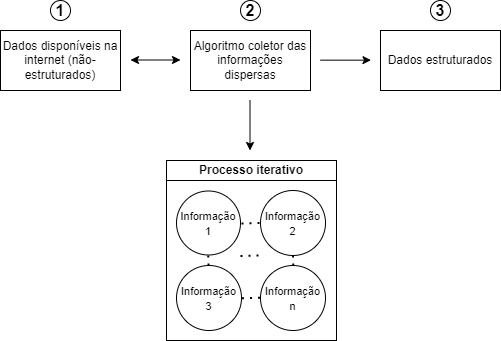
\includegraphics[scale = 0.85]{figuras/web_scraping_flow.png}
	\fonte{Elaboração do autor. Adaptado de \citeonline[p.~96]{hc_costa2016}}
\end{figure}

A maior parte dos dados disponíveis na internet possuem um arcabouço que não muda ao longo do tempo, apesar das informações contidas dentro do mesmo mudarem. O algoritmo de raspagem de dados \textit{web}, interagindo com os sites, localiza as informações, extrai os dados relevantes, estrutura e armazena os mesmos em formato painel, possibilitando futuras consultas.

Isto posto, a Figura \ref{figure:fluxo_web_scrap} nos permite observar o fluxo iterativo do coletor de dados, onde primeiro o algoritmo interpreta a esquematização da página \textit{web}. Por seguinte, iterativamente acessa o site, coletando as informações pré-definidas, extraindo os dados com base na disposição de como estão disponíveis. Essa dinâmica se repercute até que todos os dados foram coletados \cite{hc_costa2016}.

O uso desta técnica nos permite obter um grande volume de dados de forma estruturada, não só poupando tempo, como também permitindo a escalabilidade. Além disso, guarda as informações em um formato organizado, promovendo a reprodutibilidade, um princípio importante no método científico.

\subsubsection{Análise de sentimentos}

Diversas aplicações de análises de sentimento vem sendo desenvolvidas ao longo dos anos, levando em consideração que técnicas de mineração textual permitem a conversão de informações qualitativas em informações quantitativas estruturadas, facilitando a relação com pesquisas de cunho econômico, permitindo incorporá-las na modelagem econométrica. Como tratam \citeonline{liu2010sentiment_subjectivity}, a análise de sentimentos possui como principal objetivo definir técnicas automáticas para se extrair informações subjetivas de textos em linguagem natural para categorizar e identificar sentimentos em textos de forma estruturada para que possa ser utilizado por um sistema de apoio ou tomador de decisão.

A determinação do sentimento está intimamente relacionada ao formato como o texto é escrito, em que a partir de um conjunto de palavras, é possível estabelecer sua tonalidade. A maioria das abordagens de análises de sentimentos baseiam-se em dicionários léxicos, que são listas extensas de palavras que são categorizadas como positivas ou negativas de acordo com sua orientação semântica \cite{liu2010sentiment_subjectivity}.

A criação e validação dessas listas de palavras pode-se definir como um dos métodos mais robustos e confiáveis para a geração de dicionários léxicos, entretanto também é uma das maneiras que mais requisitam tempo. Dessa forma, diversas pesquisas aplicadas no tocante de análise de sentimentos baseia-se em dicionários léxicos previamente criados \cite{hutto2014vader}.

Um dos dicionários léxicos mais antigos criado foi introduzido por \citeonline{stone_etal1966}, denominado \textit{General Inquirer}, onde foi escrito manualmente. Foi desenvolvido como ferramenta para \textit{análise de conteúdo}, técnica usada por cientistas sociais, cientistas políticos e psicólogos para identificação objetiva de características específicas de mensagens. Dentre o total de palavras, 1915 categorizam-se como positivas e 2291 categorizam-se como negativas \cite{hutto2014vader}.

Ainda, tem-se que a semântica de um documento de texto é de extrema importância para sua análise, onde existem diversas técnicas para se lidar com a questão da semântica, podendo ser citadas a remoção de \textit{stopwords} e remoção de palavras e caracteres sem relevância. Muitos tipos de palavras não agregam de forma pertinente para o sentido de um documento textual, como preposições e conjunções, aparecendo repetidamente diversas vezes, podendo prejudicar o algoritmos de processamento de textos. Essas palavras são chamadas de \textit{stopwords} e, na etapa de limpeza dos dados, elas são removidas.

\subsubsubsection{A estatística tf-idf (term frequency-inverse document frequency)}

Uma das maneiras costumeiras de representar-se um texto é dividi-lo em \textit{tokens}, isto é, em palavras e outros elementos que deseja-se mapear no processamento de um documento. Conforme enunciam \citeonline{salton1975document_indexing}, entende-se que um documento é um conjunto de termos indexados que podem possuir pesos a partir da importância desse termo no documento, sendo assim pode-se representar Um documento como um vetor de $n$ dimensões como:

\begin{ceqn}
\begin{align} \label{eq:document_to_corpus}
D_{i} = (d_{i1}, d_{i2},...,d_{in})
\end{align}
\end{ceqn} em que $D_{in}$ representa o peso do $n$-ésimo termo. Sendo assim, tem-se que um \textit{Corpus} de documentos é um conjunto de documentos dispostos em um espaço vetorial, isto é, como se fosse um documento de documentos.

O método da estatística de \textit{term frequency-inverse document frequency} (tf-idf) consiste em considerar que a frequência dos \textit{tokens} de determinado documento importa para a elaboração da análise. 

A frequência de determinado termo em um documento é obtido através da quantidade de vezes que o termo surge, onde transforma-se cada documento em uma matriz de tuplas, sendo o primeiro elemento um determinado termo e o segundo elemento a frequência desse mesmo termo no documento. Para se ajustar a frequência dos termos no \textit{Corpus}, conforme apontam \citeonline{rajaraman2011mining}, é interessante considerar a proporcionalidade das frequências em relação ao tamanho do documento, tem-se então:

\begin{ceqn}
\begin{align} \label{eq:tf}
{tf}_{ij} = \frac{f_{ij}}{max_{k}f_{kj}}
\end{align}
\end{ceqn} onde $tf$ é a frequência do termo; $i$ é um termo em determinado documento $j$; e $k$ é o termo com maior frequência no documento. Ainda conforme \citeonline{rajaraman2011mining}, tem-se:

\begin{ceqn}
\begin{align} \label{eq:idf}
{idf}_{i} = \ln \left( \frac{N}{n_{i}} \right)
\end{align}
\end{ceqn} em que ${idf}_{i}$ é a frequência inversa de um termo $i$ que aparece $n$ vezes em $N$ documentos. Multiplicando a Equação \eqref{eq:tf} pela Equação \eqref{eq:idf}, chega-se então na estatística tf-idf de um termo $i$ em um documento $j$.

Em busca de considerar a influência de termos que são menos frequentes em um documento, entretando podem ser relevantes para a análise, calcula-se a frequência inversa do termo em determinado documento, minimizando a importância de palavras muito comuns e aumentando a importância de palavras mais raras. 

\subsection{Modelagem econométrica}

Nesta Subseção serão apresentados os processos da modelagem econométrica. Primeiramente é discursado sobre processos estocásticos e estacionariedade, apresentando os devidos testes, seguido pela apresentação do modelo VAR, que possibilita tanto verificar a causalidade de Granger, como elaborar a IRF. Após isso, são feitos testes de diagnóstico acerca de correlação serial e heterocedasticidade. Por fim, é apresentada a base de dados das atas do Copom e das variáveis macroeconômicas utilizadas na elaboração desta pesquisa.

\subsubsection{Processos aleatórios e séries estacionárias}

Conforme enunciado em \citeonline{gujarati_ecn2011}, define-se um processo aleatório como uma coleção de variáveis estocásticas ordenadas no tempo. Sendo assim, sugere-se que dados macroeconômicos, genericamente, são categorizados como processos aleatórios (denominados também como séries temporais). Da mesma maneira que se utiliza amostras de dados para efetuar inferências sobre uma determinada população, no campo de séries temporais, utiliza-se a realização do processo estocástico em questão para extrações inferenciais \cite{gujarati_ecn2011}.

De modo geral, caso a série temporal se enquadrar como estacionária, sua média e sua variância deverão ser constantes ao longo do tempo. Além disso, o valor da covariância entre dois períodos de tempo deverá depender somente da defasagem entre eles; de outro modo, a série não será estacionária. Tal processo estocástico é conhecido na literatura como fracamente estacionário \cite{gujarati_ecn2011, morettin2017estatistica}.

A partir de um modelo generalizado, pode-se representar diversas séries temporais e suas características. Sendo $Y_{t}$ um processo estocástico fracamente estacionário, como segue:

\begin{ceqn}
\begin{align} \label{eq:ts_generic_model}
 Y_{t} = \beta_{0} + \beta_{1} t + \beta_{2} Y_{t-1} + \mu_{t}
\end{align}
\end{ceqn} tem-se que $\beta_{0}$ é o coeficiente constante (de intercepto); $\beta_{1}$ é o coeficiente relacionado à medição do tempo $t$ (de tendência); $\beta_{2}$ é o coeficiente do termo autorregressivo (AR), que é a série no período anterior ($t-1$); e $\mu_{t}$ é um termo de erro do tipo ruído branco, a parte que o modelo não consegue captar \cite{gujarati_ecn2011}.

A depender dos valores obtidos para os estimadores de $\beta_{k}$, pode ser que a série temporal possua características de estacionariedade ou não. Supondo que $\mu_{t}$ seja um termo de erro do tipo ruído branco, com média igual à zero e variância $\sigma^2$ (constante); tem-se então que a série $Y_{t}$ é um passeio aleatório puro (sem deslocamento), conforme:

\begin{ceqn}
\begin{align} \label{eq:random_walk}
 Y_{t} = Y_{t-1} + \mu_{t}
\end{align}
\end{ceqn} em que $\beta_{0} = \beta_{1} = 0$ e $\beta_{2} = 1$. Constata-se que a variância da Equação \eqref{eq:random_walk} crescerá indefinitivamente conforme o aumento do tempo $t$, uma vez que $var(Y_{t}) = \sigma^2 t$, violando assim uma das condições de estacionariedade fraca \cite{gujarati_ecn2011}.

Subtraindo $Y_{t-1}$ de ambos os lados da Equação \eqref{eq:random_walk}, chega-se em:

\begin{ceqn}
\begin{align} \label{eq:rw_diff}
(Y_{t} - Y_{t-1}) = (Y_{t-1} - Y_{t-1}) + \mu_{t} \notag \\
(Y_{t} - Y_{t-1}) = \mu_{t} \notag \\
\Delta Y_{t} = \mu_{t}
\end{align}
\end{ceqn} onde $\Delta$ é chamado de operador de diferença, isto é, o valor da série no tempo $t$ subtraído do valor da série no tempo $t-1$. Assim como demonstrado por \citeonline{gujarati_ecn2011}, as primeiras diferenças de séries temporais de um passeio aleatório são estacionárias, e neste caso, são integradas de ordem 1, podendo ser representadas por $I(1)$, ou genéricamente como integradas de ordem $d \rightarrow I(d)$.

\subsubsubsection{Teste de raiz unitária de Dickey-Fuller Aumentado (ADF)}

Em modelos de séries temporais, a unidade de raiz é uma importante característica dos processos de realização da série que, caso não for adequadamente tratada, pode causar problemas de inferência. Reescrevendo a Equação \eqref{eq:random_walk} como:

\begin{ceqn}
\begin{align} \label{eq:rw_rho}
 Y_{t} = \rho Y_{t-1} + \mu_{t} \qquad (-1 \leq \rho \leq 1)
\end{align}
\end{ceqn} tem-se $\mu_{t}$ como termo de erro ruído branco; e $\rho$ como coeficiente de autocorrelação entre $Y_{t}$ e $Y_{t-1}$. Caso $\rho = 1$, a Equação \eqref{eq:rw_rho} será um processo de passeio aleatório e se terá problema de raiz unitária, ou seja, problema de estacionariedade na série. Subtraindo $Y_{t-1}$ de ambos os lados da Equação \eqref{eq:rw_rho} e aplicando o operador de diferença, é possível chegar em:

\begin{ceqn}
\begin{align} \label{eq:df_test}
Y_{t} - Y_{t-1} = \rho Y_{t-1} - Y_{t-1} + \mu_{t} \notag \\
\Delta Y_{t} = (\rho - 1) Y_{t-1} + \mu_{t} \notag \\
\Delta Y_{t} = \delta Y_{t-1} + \mu_{t}
\end{align}
\end{ceqn} em que $\delta = (\rho - 1)$.

Para se efetuar o teste de raiz unitária, deve-se estimar os parâmetros da Equação \eqref{eq:df_test}, testando a hipótese nula ($H_{0})$) contra a hipótese alternativa ($H_{1}$), como segue:

\begin{ceqn}
\begin{align} \label{eq:hipoteses_estacionariedade}
&H_{0}: \delta = 0 \\ % \qquad \rightarrow \text{série não estacionária}
&H_{1}: \delta < 0 %\qquad \rightarrow \text{série estacionária}
\end{align}
\end{ceqn}

Caso o resultado do teste for $\delta = 0$, terá-se então um $\rho = 1$, isto é, raiz unitária. Dessa forma, o processo estócastico testado trata-se de uma série não estacionária. Como demonstrado por \citeonline{UR_dickey_fuller1979} e abordado em \citeonline{gujarati_ecn2011}, o valor estimado de $t$ para o coeficiente $Y_{t-1}$ da Equação \eqref{eq:df_test} segue a estatística $\tau$ (tau). Os valores fundamentais da estatística $\tau$ foram computadas a partir de simulações de Monte Carlo, onde o teste ficou conhecido como teste de Dickey-Fuller. Com o objetivo de englobar diversas possibilidades, a estimação do teste é feito de três formas:

\begin{ceqn}
\begin{align} \label{eq:df_equations}
&\Delta Y_{t} = \delta Y_{t-1} + \mu_{t} \qquad \qquad \qquad \qquad \qquad \qquad \qquad \text{\textbf{(passeio aleatório)}} \\
&\Delta Y_{t} = \beta_{0} + \delta Y_{t-1} + \mu_{t} \qquad \qquad \qquad \text{\textbf{(passeio aleatório com deslocamento)}} \\
&\Delta Y_{t} = \beta_{0} + \beta_{1} t + \delta Y_{t-1} + \mu_{t} \quad \text{\textbf{(passeio aleatório com deslocamento e tendência)}} 
\end{align}
\end{ceqn}

A estatística tau calculada ($\tau_{calculada}$) pode ser obtida ao dividir o delta estimado ($\hat{\delta}$) pelo seu desvio-padrão ($\sigma_{\hat{\delta}}$), e caso seu módulo for maior do que o módulo da estatística tau crítica (|$\tau_{critica}$|), se rejeita a hipótese nula ($H_{0}$) de que não há estacionariedade, caso contrário, trata-se de uma série estacionária.

Para as situações em que os resíduos da série temporal ($\mu_{t}$) são correlacionados, ou seja, problema de autocorrelação, utiliza-se do teste de Dickey-Fuller Aumentado (ADF), em que trata de adicionar valores defasados da variável $Y_{t}$ na estimação, chegando-se na seguinte equação:

\begin{ceqn}
\begin{align} \label{eq:adf_equation}
\Delta Y_{t} = \beta_{0} + \beta_{1} t + \delta Y_{t-1} + \sum_{p=1}^{n}{\alpha_{p} \Delta Y_{t-p}} + \epsilon_{t}
\end{align}
\end{ceqn} em que $\epsilon_{t}$ é um termo de ruído branco e $p_{1,...,n}$ refere-se ao número de defasagens. 

O objetivo é adicionar termos suficientes na Equação \eqref{eq:adf_equation} de maneira que o erro $\epsilon_{t}$ seja serialmente não correlacionado, para que seja possível obter-se uma estimativa não viesada de $\delta$, que é o coeficiente defasado de $Y_{t-1}$. Embora haver mais parâmetros no teste de Dickey-Fuller Aumentado, ainda é testado se $\delta = 0$, seguindo a mesma distribuição assintótica da estatística de Dickey-Fuller, de forma que os mesmos valores de $\tau$ podem ser utilizados \cite{gujarati_ecn2011}.

Dada determinada ordem de defasagem máxima ($\rho_{maxima}$), a partir do critério de informação de Akaike (AIC) ou critério Bayesiano de Schwarz (BIC), pode-se selecionar a melhor extensão de defasagens para o modelo. Conforme apresentado em \citeonline{bueno2008}, a escolha do número máximo máximo de extensões dá-se pelo número inteiro obtido atráves de:

\begin{ceqn}
\begin{align} \label{eq:rho_max}
\rho_{maxima} = 12 \left(\frac{N}{100}\right)^\frac{1}{4}
\end{align}
\end{ceqn} em que $N$ é o tamanho da amostra. Dado um nível de significância ($\alpha$) de $5,00$\%, exibe-se na Tabela \ref{table:tabela_tau} os valores críticos para a estatística $\tau$.

\begin{table}[hbtp]
	\centering
	\caption{Valores críticos para a estatística $\tau$ dado um $\alpha = 5,00$\%} \label{table:tabela_tau}
	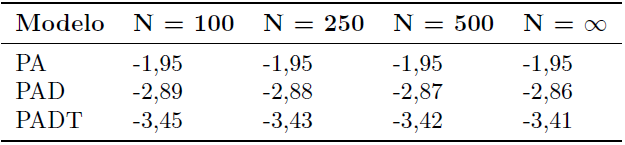
\includegraphics[scale = 0.75]{figuras/tabela_tau.PNG}
	\fonte{Elaboração do autor. Adaptado de \citeonline{fuller1976}.} 
\end{table}

Como ponto de observação, na primeira coluna, PA refere-se à passeio aleatório (sem constante), PAD refere-se à passeio aleatório com deslocamento (com constante) e PADT refere-se à passeio aleatório com deslocamento e tendência (com constante e tendência).

\subsubsubsection{Teste de raiz unitária de Phillips-Perron (PP)}

Outro teste conhecido é o teste desenvolvido por \citeonline{UR_phillips_perron1988}, em que propõem um método alternativo e não-paramétrico de controlar a autocorrelação ao testar-se a raiz unitária, permitindo que seja consistente mesmo havendo variáveis dependentes defasadas e correlação serial nos resíduos. Sendo assim, o teste de Phillips-Perron (PP) faz com que seja desnecessária a especificação de um modelo com ordem suficientemente autorregressivo para a eliminação do problema de autocorrelação \cite{bueno2008}.

Considerando a seguinte alternativa de regressão $\Delta Y_{t}$ e a sua respectiva estatística $Z_{t}$ associada, tem-se:

\begin{ceqn}
\begin{align} \label{eq:pp_1}
%&\Delta Y_{t} = \alpha Y_{t-1} + \mu_{t} \qquad \qquad \qquad \rightarrow Z_{t} \nonumber \\
\Delta Y_{t} = \omega + \alpha Y_{t-1} + \mu_{t} \qquad \rightarrow \qquad Z_{t, \omega} 
%&\Delta Y_{t} = \omega + \delta t + \alpha Y_{t-1} + \mu_{t} \qquad \rightarrow Z_{t, \tau} \nonumber
\end{align}
\end{ceqn} em que $\Delta$ é o operador da diferença e $\mu_{t}$ é um processo estacionário. Estima-se então o parâmetro $\hat{\alpha}$ de interesse:

\begin{ceqn}
\begin{align} \label{eq:pp_alpha}
\hat{\alpha} = \frac{\sum_{t=1}^{N}{(Y_{t-1} - \overline{Y}_{-1}) (Y_{t} - \overline{Y})}}{\sum_{t=1}^{N}{(Y_{t-1} - \overline{Y}_{-1})^2}} - 1
\end{align}
\end{ceqn} onde $\overline{Y}$ representa a média, sendo possível estimar a variância populacional $\hat{\sigma}^2$:

\begin{ceqn}
\begin{align} \label{eq:pp_sigma}
\hat{\sigma}^2 = \frac{\sum_{t=1}^{N}{(\Delta Y_{t} - \hat{\omega} - \hat{\alpha} Y_{t-1})^2}}{N}
\end{align}
\end{ceqn} e a partir da Equação \eqref{eq:pp_sigma} pode-se calcular a variância de longo prazo $\hat{\upsilon}^2$:

\begin{ceqn}
\begin{align} \label{eq:pp_vega}
\hat{\upsilon}^2 = \hat{\sigma}^2 + \frac{2}{N} \sum_{j=1}^{M}{\phi \left(\frac{j}{M+1} \right)} \sum_{t=j+1}^{N}{\hat{\mu}_{t} \hat{\mu}_{t-j}}
\end{align}
\end{ceqn} podendo-se chegar afinal na estatística de PP, dada por:

\begin{ceqn}
\begin{align} \label{eq:pp_total}
\hat{Z}_{t, \omega} = \hat{\tau}_{\omega} \left(\frac{\hat{\sigma}}{\hat{\upsilon}} \right) - \frac{1}{2} \left(\frac{\hat{\upsilon}^2 - \hat{\sigma}^2}{\hat{\upsilon} \sqrt{N^{-2} \sum_{t=1}^{N} Y_{t-1}^2}} \right)
\end{align}
\end{ceqn} em que na variância de longo prazo estão inclusas todas as autocovariâncias do processo $\mu_{t}$.

A interpretação do teste de PP é a mesma do que a do teste de ADF, uma vez que possuem a mesma distribuição assintótica, tendo-se que a hipótese nula ($H_{0}$) é de que a série apresenta raiz unitária contra a hipótese alternativa ($H_{1}$) de que a série é estacionária \cite{bueno2008, gujarati_ecn2011}.

\subsubsubsection{Teste de raiz unitária de Kwiatkowski–Phillips–Schmidt–Shin (KPSS)}

Devido à facilidade de implementação e bom funcionamento dos testes de raiz unitária ADF e PP, eles são popularmente utilizados. Entretanto, tanto o teste ADF quanto o teste de PP possuem como $H_{0}$ a presença de raiz unitária, isto é, a não estacionariedade. De qualquer maneira, a literatura acerca do tema frequentemente aceita a $H_{1}$, caso inexistam evidências contrárias a $H_{0}$, ainda mais quando trata-se de séries macroeconômicas. Devido a esse fator, faz-se de bom uso a aplicação de um teste que tenha como $H_{0}$ a estacionariedade e outro que a tenha como $H_{1}$ \cite{kennedy2008guide_to_econometrics}.

O teste desenvolvido por \citeonline{UR_kpss1992}, conhecido como teste KPSS (mnemônico dos autores), possui a estacionariedade da série como hipótese nula ($H_{0}$), frente a não estacionariedade como hipótese alternativa ($H_{1}$), como segue:

\begin{ceqn}
\begin{align} \label{eq:hipoteses_kpss}
&H_{0}: Y_{t} \thicksim I(0) \\
&H_{1}: Y_{t} \thicksim I(1) 
\end{align}
\end{ceqn}

O objetivo é usar o teste como complementar aos testes tradicionais, distinguindo assim a raiz unitária de séries cujos dados não são suficientemente conclusivos (como séries macroeconômicas), caracterizando-se assim mais assertivamente a série \cite{bueno2008}.

O teste KPSS decompõe a série em questão em três partes, conforme:

\begin{ceqn}
\begin{align} \label{eq:kpps_ts_1}
Y_{t} = \eta t + \phi_{t} + \epsilon_{t}
\end{align}
\end{ceqn} onde $\eta t$ é o elemento de tendência determinística, $\phi_{t}$ é o elemento de passeio aleatório e $\epsilon_{t}$ é o elemento de erro estacionário. É efetuado então um processo de soma parcial dos resíduos, como:

\begin{ceqn}
\begin{align} \label{eq:kpps_ts_2}
S_{t} = \sum_{t=1}^{N}{\hat{e}_{t}}
\end{align}
\end{ceqn} no qual $\hat{e}_{t}$ são os erros da Equação \eqref{eq:kpps_ts_1}. Tendo a variância de longo prazo ($\hat{\upsilon}^2$) como definida na Equação \eqref{eq:pp_sigma}, chega-se à estatística do teste KPSS, dada por:

\begin{ceqn}
\begin{align} \label{eq:stat_kpss}
KPSS = \sum_{t=1}^{N}{\frac{S_{t}^2}{N^2 \hat{\upsilon}^2}}
\end{align}
\end{ceqn}

Caso $Y_{t}$ for um processo estacionário, então $S_{t} \thicksim I(1)$ e o numerador da estatística KPSS será um estimador da variância de $S_{t}$, tendo assim um limite assintótico. Já o denominador observado na Equação \eqref{eq:stat_kpss} assegura que a distribuição seja livre de ruídos. Na outra mão, caso $Y_{t} \thicksim I(1)$, o numerador crescerá ilimitadamente, fazendo a estatística KPSS ficar muito elevada.  \cite{bueno2008}.

Compara-se então a estatística calculada com os valores críticos a determinado nível de significância, sendo que se o valor calculado for maior que o valor crítico, rejeita-se a $H_{0}$ de estacionariedade. Os valores críticos para a realização do teste de KPSS, que foram calculados e apresentados em \citeonline{UR_kpss1992}, são utilizados como parâmetros de comparação.

Já em relação a ordem de defasagem máxima ($\rho_{maxima}$) na regressão, como apontado em \citeonline{tseries2022R_package}, será utilizado o número inteiro obtido através de:

\begin{ceqn}
\begin{align} \label{eq:rho_max_kpss}
\rho_{maxima} = 4 \left( \frac{N}{100} \right)^\frac{1}{4}
\end{align}
\end{ceqn} alternativamente à Equação \eqref{eq:rho_max}.

\subsubsection{Vetores autorregressivos (VAR)}

A modelagem econômica em geral é caracterizada por haver diversas variáveis, sendo assim, modelos univariados são limitados para expressar modelos econômicos. O VAR permite que sejam expressos modelos econômicos e se estimem seus parâmetros. Genericamente falando, pode-se definir um modelo autorregressivo de ordem $p$, isto é, um VAR($p$) como:

\begin{ceqn}
\begin{align} \label{eq:var_1}
A Y_{t} = B_{0} + \sum_{i=1}^{p}{B_{i} Y_{t-i}} + \epsilon_{t}
\end{align}
\end{ceqn} onde $A$ representa uma matriz $n \times n$ que define as restrições contemporâneas; $Y_{t}$ é um vetor $n \times 1$ das variáveis endógenas no período $t$; $B_{0}$ é um vetor de constantes $n \times 1$; $B_{i}$ é uma matriz $n \times n$ dos parâmetros referentes ao vetor $Y_{t-i}$, que são as variáveis endógenas defasadas $i$ vezes, possuindo dimensão $n \times 1$; e por fim $\epsilon_{t}$ é um vetor $n \times 1$ de erros do tipo ruído branco \cite{bueno2008}.

A Equação \eqref{eq:var_1} demonstra as relações entre as variáveis endógenas em sua forma estrutural, onde os choques $\epsilon_{t}$ são chamados de choques estruturais, uma vez que afetam de forma individual cada uma das variáveis endógenas. Por causa disso, o modelo costumeiramente é estimado na sua forma reduzida, multiplicando a equação por $A^{-1}$, conforme:

\begin{ceqn}
\begin{align} \label{eq:var_2}
Y_{t} = A^{-1} B_{0} + \sum_{i=1}^{p}{A^{-1} B_{i} Y_{t-i}} + A^{-1} \epsilon_{t}
\end{align}
\end{ceqn} onde $C \equiv A^{-1} B_{0}$; $\phi_{i} \equiv A^{-1} B_{i}$ e $e_{t} \equiv A^{-1} \epsilon_{t}$, chegando-se então em:

\begin{ceqn}
\begin{align} \label{eq:var_3}
Y_{t} = C + \sum_{i=1}^{p}{\phi_{i} Y_{t-i}} + e_{t}
\end{align}
\end{ceqn}

Convenientemente, conforme \citeonline{enders2008econometrics}, será considerado o modelo disposto na Equação \eqref{eq:var_3} como um modelo bivariado com defasagem de ordem igual a 1, chegando no sistema:

\begin{ceqn}
\begin{align} \label{eq:var_4}
&y_{t} = b_{10} - a_{12} z_{t} + b_{11} y_{t-1} + b_{12} z_{t-1} + \sigma_{y} \epsilon_{yt} \\
&z_{t} = b_{20} - a_{21} y_{t} + b_{21} y_{t-1} + b_{22} z_{t-1} + \sigma_{z} \epsilon_{zt}
\end{align}
\end{ceqn}

Nota-se que as variáveis são mutuamente influenciadas umas pelas outras, tanto com seus valores atuais quanto com seus valores defasados. O VAR não pode ser diretamente estimado, considerando que as variáveis atuais $z_{t}$ e $y_{t}$ são isoladamentes correlacionadas aos erros $\epsilon_{yt}$ e $\epsilon_{zt}$, respectivamente. Isso acontece, pois cada uma dessas variáveis depende do comportamento da outra, tendo como objetivo do VAR encontrar a trajetória da variável de interesse a partir da efetuação de um choque nesses erros \cite{bueno2008}.

\subsubsubsection{Causalidade de Granger}

A causalidade no sentido de Granger acontece quando uma variável é capaz de prever outra variável e em sob quais condições, isto é, quando é possível utilizar uma variável, seja defasada ou não, para prever outra variável em determinado período de tempo. O objetivo é determinar se $y$ ajuda a prever $z$ e caso isso não aconteça, tem-se que $y$ não Granger-causa $z$. O teste feito então é:

\begin{ceqn}
\begin{align} \label{eq:granger_causality}
z_{t} = \phi_{20} + \sum_{i=1}^{p}{\phi_{i, 21} y_{t-i}} + \sum_{i=1}^{p}{\phi_{i, 22} z_{t-i}} + e_{2t}
\end{align}
\end{ceqn} onde a seguinte hipótese nula ($H_{0}$) é testada frente a hipótese alternativa ($H_{1}$):

\begin{ceqn}
\begin{align} \label{eq:granger_causality_hip}
&H_{0}: \phi_{i, 21} = 0 \qquad \text{(ausência de Granger-causalidade)}\\
&H_{1}: \phi_{i, 21} \neq 0 \qquad \text{(presença de Granger-causalidade)}
\end{align}
\end{ceqn} em que a estatística do teste ($S_{1}$) é dada por:

\begin{ceqn}
\begin{align} \label{eq:granger_causality_stat}
S_{1} = \frac{\frac{(e_{\gamma}^2 - e_{\mu}^2)}{p}}{\frac{e_{\mu}^2}{N - 2p - 1}} \qquad \rightarrow \qquad F(p; N - 2p - 1)
\end{align}
\end{ceqn} tal qual $\gamma$ representa restrito e $\mu$ representa irrestrito. 

Caso $S_{1} > F$ dado um nível de significância ($\alpha$), rejeita-se a hipótese nula de que $y$ não Granger-causa $z$, ou seja, se conclui que existe uma relação de causalidade no sentido de Granger \cite{bueno2008, gujarati_ecn2011}.

Para se definir a quantidade ideal de defasagens a serem inseridas dentro do sistema de equações, pode-se utilizar os critérios de informação, em que atribuem penalidade conforme aumenta-se o número de regressores, por impactar na soma dos resíduos do modelo. Estes critérios então minimizam uma função que baseia-se nos resíduos da regressão estimada, penalizada pela quantidade de regressores que foram utilizados \cite{bueno2008}.

O modelo mais ideal será o com maior parcimônia, isto é, com menor número de parâmetros, satisfazendo com que os resíduos sejam os menores possíveis. Geralmente, o critério de especificação possui o seguinte formato:

\begin{ceqn}
\begin{align} \label{eq:general_inf_crit}
CE = \ln \hat{\sigma}^2 (N) + c_{N} \varphi (N)
\end{align}
\end{ceqn} onde $\hat{\sigma}^2 (N) = \frac{\sum_{t=1}^{N}{\hat{\epsilon}_{t}^2}}{N} $ é a variância estimada dos resíduos; $c_{N}$ é o número de parâmetros estimados; e $\varphi (N)$ é a ordem do processo, que penaliza a falta de parcimoniosidade. Dessa forma, existem três principais critérios de informação, onde a estatística de Critério de Informação Bayesiano (BIC) se dá por:

\begin{ceqn}
\begin{align} \label{eq:BIC}
BIC(p,q) = \ln \hat{\sigma}^2 + n \frac{ln N}{N}
\end{align}
\end{ceqn} no qual $n = p + q$ caso o modelo não possuir constante ou $n = p + q + 1$ caso houver constante.

Outro critério é a estatística de Critério de Informação de Akaike (AIC), em que:

\begin{ceqn}
\begin{align} \label{eq:AIC}
AIC(p,q) = \ln \hat{\sigma}^2 + n \frac{2}{N}
\end{align}
\end{ceqn}

Por fim, a estatística Hannan-Quinn (HQ) é conforme segue:

\begin{ceqn}
\begin{align} \label{eq:HQ}
HQ(p,q) = \ln \hat{\sigma}^2 + n \frac{2}{N} \ln (\ln N)
\end{align}
\end{ceqn}

A primeira parte da Equação \eqref{eq:general_inf_crit} mede a adequação do processo, em que quanto menor a variância dos resíduos, melhor. Entretanto, uma redução de variância que foi obtida ao introduzir mais parâmetros é penalizada pela segunda parte da equação. Dessa maneira, deseja-se o menor AIC, BIC ou HQ possível \cite{bueno2008}.

\subsubsubsection{Função de impulso-resposta (IRF)}

Assim como existe a possibilidade de se retratar um modelo autorregressivo como seu componente de média móvel, pode-se representar um modelo VAR($p$) como um Vetor de Média Móvel (VMA), isto é, um VMA($\infty$). Dessa forma, como abordado em \citeonline{sims1980macroeconomics}, elabora-se projeções distintas a partir da efetuação de choques nas variáveis introduzidas no modelo VAR($p$). Considerando uma abordagem matricial para um modelo de VAR($1$), tem-se:

\begin{ceqn}
\begin{align} \label{eq:mat_var}
\begin{bmatrix}
y_{1t} \\
y_{2t}
\end{bmatrix}
=
\begin{bmatrix}
\alpha_{1} \\
\alpha_{2}
\end{bmatrix}
+
\begin{bmatrix}
\phi_{11} y_{1, t-1} \\
\phi_{12} y_{1, t-1}
\end{bmatrix}
+
\begin{bmatrix}
\phi_{21} y_{2, t-1} \\
\phi_{22} y_{2, t-1}
\end{bmatrix}
+
\begin{bmatrix}
\mu_{1t} \\
\mu_{2t}
\end{bmatrix}
\end{align}
\end{ceqn} no qual, reescrevendo a Equação \eqref{eq:mat_var}, chega-se em:

\begin{ceqn}
\begin{align} \label{eq:mat_var_2}
\begin{bmatrix}
y_{1t} \\
y_{2t}
\end{bmatrix}
=
\begin{bmatrix}
\overline{y}_{1} \\
\overline{y}_{2}
\end{bmatrix}
+
\sum_{i=0}^{\infty}{\begin{bmatrix} \phi_{11} & \phi_{12} \\ \phi_{21} & \phi_{22} \end{bmatrix}^i}
\begin{bmatrix}
\mu_{1, t-i} \\
\mu_{2, t-i}
\end{bmatrix}
\end{align}
\end{ceqn} em que a Equação \eqref{eq:mat_var_2} representa $\begin{bmatrix} y_{1t} \\ y_{2t} \end{bmatrix}$ em termos de $\begin{bmatrix} \mu_{1t} \\ \mu_{2t} \end{bmatrix}$. Entretranto, reescrevendo em relação a $\begin{bmatrix} \mu_{y_{1}t} \\ \mu_{y_{2}t} \end{bmatrix}$, conforme aborda \citeonline{enders2008econometrics}, obtém-se:

\begin{ceqn}
\begin{align} \label{eq:mat_var_3}
\begin{bmatrix}
\mu_{1t} \\
\mu_{2t}
\end{bmatrix}
=
\frac{1}{1-b_{12}b_{21}} \begin{bmatrix} 1 & -b_{12} \\ -b_{21} & 1 \end{bmatrix}
\begin{bmatrix}
\mu_{y_{1}t} \\
\mu_{y_{2}t}
\end{bmatrix}
\end{align}
\end{ceqn} onde ao combinar a Equação \eqref{eq:mat_var_2} e a Equação \eqref{eq:mat_var_3}, terá-se:

\begin{ceqn}
\begin{align} \label{eq:mat_var_4}
\begin{bmatrix}
y_{1t} \\
y_{2t}
\end{bmatrix}
=
\begin{bmatrix}
\overline{y}_{1} \\
\overline{y}_{2}
\end{bmatrix}
+
\frac{1}{1-b_{12}b_{21}}
\sum_{i=0}^{\infty}{\begin{bmatrix} \phi_{11} & \phi_{12} \\ \phi_{21} & \phi_{22} \end{bmatrix}^i}
\begin{bmatrix} 1 & -b_{12} \\ -b_{21} & 1 \end{bmatrix}
\begin{bmatrix}
\mu_{y_{1}t} \\
\mu_{y_{2}t}
\end{bmatrix}
\end{align}
\end{ceqn} em que, para simplificar, define-se a matriz $\Theta_{i}$ como:

\begin{ceqn}
\begin{align} \label{eq:irf}
\Theta_{i} = \frac{A_{1}^i}{1-b_{12}b_{21}} \begin{bmatrix} 1 & -b_{12} \\ -b_{21} & 1 \end{bmatrix}
\end{align}
\end{ceqn} e com isso, a representação de média móvel introduzida na Equação \eqref{eq:mat_var_2} pode ser reescrita conforme:

\begin{ceqn}
\begin{align} \label{eq:irf_2}
\begin{bmatrix}
y_{1t} \\
y_{2t}
\end{bmatrix}
=
\begin{bmatrix}
\overline{y}_{1} \\
\overline{y}_{2}
\end{bmatrix}
+
\sum_{i=0}^{\infty}{\begin{bmatrix} \Theta_{11}(i) & \Theta_{12}(i) \\ \Theta_{21}(i) & \Theta_{22}(i) \end{bmatrix}^i}
\begin{bmatrix}
\mu_{y_{1}t} \\
\mu_{y_{2}t}
\end{bmatrix}
\end{align}
\end{ceqn} sendo assim, de maneira mais compacta:

\begin{ceqn}
\begin{align} \label{eq:irf_3}
Y_{t} = \overline{Y}_{t} + \sum_{i=0}^{\infty}{\Theta_{i} \mu_{t-i}}
\end{align}
\end{ceqn} em que os elementos da matriz $\Theta_{i}$ são denominados multiplicadores de impacto de um choque sobre as variáveis endógenas. Dessa forma, o impacto total de um choque de $\mu_{y_{1}t}$ sobre $Yt_{t+n}$ é dado por $\sum_{i=0}^{n}{\Theta_{11}(i)}$, sendo que caso $y_{1}$ e $y_{2}$ forem estacionárias, os valores de $\Theta_{xz}(i)$ convirjirão para zero conforme aumentar-se $i$, implicando que os choques não possuem efeitos permanentes em séries estacionárias \cite{bueno2008}.

\subsubsection{Autocorrelação serial}

Define-se autocorrelação serial como a correlação entre o termo de erro $\mu$ em determinado período $t$ e o termo de erro $\mu$ em seu período anterior $t-1$, isto é, a relação de $\mu_{t}$ e $\mu_{t-1}$. Levando em consideração uma série temporal na forma:

\begin{ceqn}
\begin{align} \label{eq:ts_autocorrel}
 Y_{t} = \beta_{0} + \beta_{1} X_{t} + \mu_{t}
\end{align}
\end{ceqn} supõe-se que o termo de erro $\mu_{t}$ é gerado pelo mecanismo:

\begin{ceqn}
\begin{align} \label{eq:ts_residual}
\mu_{t} = \lambda \mu_{t-1} + \epsilon_{t} \qquad (-1 < \lambda < 1)
\end{align}
\end{ceqn} em que $\lambda$ é o coeficiente de autocovariância e $\epsilon_{t}$ é o termo de erro estocástico, ao qual atende à hipótese padrão dos Mínimos Quadrados Ordinários (MQO):

\begin{ceqn}
\begin{align} \label{eq:ts_error_white_noise}
&E(\epsilon_{t}) = 0 \nonumber \\
&var(\epsilon_{t}) = \sigma^2 \\
&cov(\epsilon_{t}, \epsilon_{t+s}) = 0 \qquad (s \neq 0) \nonumber
\end{align}
\end{ceqn} sendo que por possuir tais propriedades, o termo de erro $\epsilon_{t}$ é denominado de ruído branco.

A Equação \eqref{eq:ts_residual} é conhecida como processo autorregressivo de primeira ordem de Markov e aponta que o valor do erro no período atual $t$ depende de uma proporção $\lambda$ do seu valor no período anterior, somado de um termo de erro totalmente aleatório $\epsilon_{t}$ \cite{gujarati_ecn2011}.

\subsubsubsection{Teste de Durbin-Watson (DW)}

Para verificação da existência - e se cabível o grau - de autocorrelação, um popular teste que é empregado é a estatística $d$ introduzida por \citeonline{durbin_watson1950}, definida como:

\begin{ceqn}
\begin{align} \label{eq:durbin_watson}
d = \frac{\sum{\hat{\mu}_{t}^2} + \sum{\hat{\mu}_{t-1}^2} - 2 \sum{\hat{\mu}_{t} \hat{\mu}_{t-1}}}{\sum{\hat{\mu}_{t}^2}} 
\end{align}
\end{ceqn} considerando que $\sum{\hat{\mu}_{t}^2} \approx \sum{\hat{\mu}_{t-1}^2}$, tem-se então:

\begin{ceqn}
\begin{align} \label{eq:durbin_watson_2}
d \approx 2 \left( 1 - \frac{\sum{\hat{\mu}_{t} \hat{\mu}_{t-1}}}{\sum{\hat{\mu}_{t}^2}} \right)
\end{align}
\end{ceqn} em que $\approx$ significa aproximadamente. Definindo:

\begin{ceqn}
\begin{align} \label{eq:dw_lambda}
\hat{\lambda} = \frac{\sum{\hat{\mu}_{t} \hat{\mu}_{t-1}}}{\sum{\hat{\mu}_{t}^2}}
\end{align}
\end{ceqn} pode-se expressar a Equação \eqref{eq:durbin_watson_2} como:

\begin{ceqn}
\begin{align} \label{eq:durbin_watson_3}
d \approx 2 (1 - \hat{\lambda})
\end{align}
\end{ceqn} onde $\hat{\lambda}$ é o coeficiente de covariância estimado da Equação \eqref{eq:ts_residual}.

Considerando que $-1 < \lambda < 1$, a Equação \eqref{eq:durbin_watson_3} denota que $0 \leq d \leq 4$. Valores próximos de zero para a estatística $d$ indicam correlação positiva, ficando próximo de 2 de acordo com menor evidência de autocorrelação. 

A Figura \ref{figure:intervalos_dw} apresenta as regras de decisão determinadas por \citeonline{durbin_watson1950}, em que $d_{L}$ denota o limite inferior da estatística $d$ e $d_{U}$ denota o limite superior da estatística $d$.

\begin{figure}[hbtp]
	\centering
	\caption{Zonas da estatística $d$ de Durbin-Watson} \label{figure:intervalos_dw}
	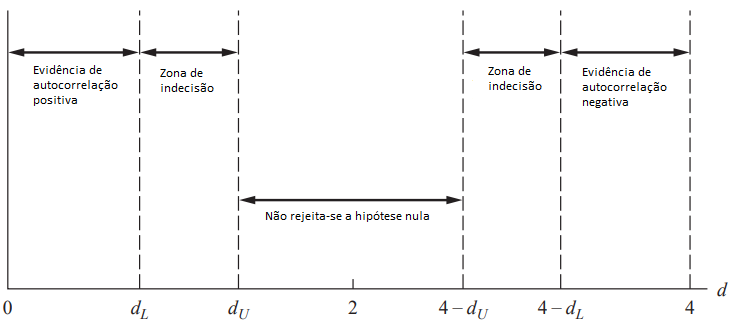
\includegraphics[scale = 0.65]{figuras/figura_durbin_watson.PNG}
	\fonte{Elaboração do autor. Adaptado de \citeonline{gujarati_ecn2011}.}
\end{figure}

É testado então a hipótese nula ($H_{0}$) contra a hipótese alternativa ($H_{1}$), tal qual:

\begin{ceqn}
\begin{align} \label{eq:hipoteses_autocorrelacao}
&H_{0}: \text{nenhuma autocorrelação, positiva ou negativa} \\
&H_{1}: \text{presença de autocorrelação}
\end{align}
\end{ceqn}

Salienta-se que $d_{L}$ e $d_{U}$ dependem do tamanho da amostra e da quantidade de variáveis explicativas do modelo; e caso $d_{U} < d < (4 - d_{U})$, não rejeita-se a hipótese nula ($H_{0}$) de ausência de autocorrelação serial \cite{gujarati_ecn2011}.

\subsubsubsection{Teste de Breusch-Godfrey (BG)}

Conforme apontado em \citeonline{gujarati_ecn2011}, para se evitar algumas armadilhas do teste $d$ de Durbin-Watson, \citeonline{breusch1978test} e \citeonline{godfrey1978test} desenvolveram um teste de autocorrelação que é genérico, não permitindo regressores não estocásticos (como valores defasados do regressando); esquemas autorregressivos de ordem superior; e médias móveis simples ou de ordem mais elevada de resíduos do tipo ruído branco, como $\epsilon_{t}$ na Equação \eqref{eq:ts_residual}.

O teste BG, também conhecido como teste do Multiplicador de Lagrange (LM), pressupõe que o termo de erro $\mu_{t}$ da Equação \eqref{eq:ts_autocorrel} siga um esquema autorregressivo de ordem $p$, como evidenciado em:

\begin{ceqn}
\begin{align} \label{eq:bg_1}
\mu_{t} = \lambda_{1} \mu_{t-1} + \lambda_{2} \mu_{t-2} + [...] + \lambda_{p} \mu_{t-p} + \epsilon_{t}
\end{align}
\end{ceqn} em que $\epsilon_{t}$ é um termo de erro do tipo ruído branco, tal qual apresentado em \eqref{eq:ts_error_white_noise}. O teste LM baseia-se em efetuar a regressão original, obtendo-se assim os resíduos estimados $\hat{\mu}_{t}$ e após isso introduzir os valores defasados dos resíduos como regressores adicionais no modelo:

\begin{ceqn}
\begin{align} \label{eq:bg_2}
\hat{\mu}_{t} = \alpha_{0} + \alpha_{1} X_{t} + \hat{\lambda}_{1} \hat{\mu}_{t-1} + \hat{\lambda}_{2} \hat{\mu}_{t-2} + [...] + \hat{\lambda}_{p} \hat{\mu}_{t-p} + \epsilon_{t}
\end{align}
\end{ceqn}

Tendo N como o tamanho da amostra e $R^2$ como o coeficiente de determinação da Equação \eqref{eq:bg_2}, \citeonline{breusch1978test} e \citeonline{godfrey1978test} demonstraram que para amostras grandes ($N \rightarrow \infty$), a relação $(N-p) R^2$ seguirá uma distribuição qui-quadrado com $p$ graus de liberdade, sendo assim:

\begin{ceqn}
\begin{align} \label{eq:chi_squared}
(N-p) R^2 \thicksim \chi_{p}^2
\end{align}
\end{ceqn}

Realiza-se então a testagem de hipóteses a determinado nível de significância ($\alpha$), tendo a hipótese nula ($H_{0}$) a ser testada como segue:

\begin{ceqn}
\begin{align} \label{eq:h0_bg_test}
H_{0}: \lambda_{1} = \lambda_{2} = [...] = \lambda_{p} = 0 \quad \rightarrow \quad \text{ausência de autocorrelação nos resíduos}
\end{align}
\end{ceqn}

Desse modo, caso $(N-p) R^2$ exceder o valor crítico ao nível determinado de $\alpha$, rejeita-se a $H_{0}$, em que pelo menos um dos $\lambda_{i}$ na Equação \eqref{eq:bg_2} é estatísticamente significantemente diferente de zero \cite{gujarati_ecn2011, bueno2008}.

O fato de uma série possuir autocorrelação faz com que a eficiência dos esimadores de MQO seja afetada, subestimando assim a variância - e por consequência, os erros padrão - do modelo. Contudo, estimadores MQO permanecem não tedenciosos, convergindo assim para seu valor populacional verdadeiro \cite{gujarati_ecn2011}.

\subsubsection{Heterocedasticidade da variância dos resíduos}

Não só autocorrelação serial é um problema, como os resíduos de determinada regressão podem ser heterocedásticos, isto é, sua variância não será constante ao longo do tempo (indiferentemente dos valores assumidos pela(s) variável(is) independente(s)). Os fatos de linearidade e parâmetros do modelo não serem tendenciosos não são alterados pela aparição de heterocedasticidade nas estimativas, apesar disso, caso tiver-se resíduos que forem heterocedásticos, terá-se perda de eficiência, uma vez que distorcem as variâncias do modelo e dos estimadores \cite{gujarati_ecn2011}.

Assim como é levantado em \citeonline{gujarati_ecn2011}, diversos testes de heterocedasticidade foram propostos com o decorrer dos anos, podendo ser citados o teste de \citeonline{park1966heterocedast}, o teste de \citeonline{glejser1969heterocedast}, o teste de \citeonline{goldfeld_quandt1972heterocedast}, o teste de \citeonline{breusch_pagan1979heterocedast} e o teste geral de \citeonline{white1980heterocedast}.

%\subsubsubsection{Teste geral de White}

%Entretanto, o teste mais popular é conhecido como o teste geral de heterocedasticidade de \citeonline{white1980heterocedast}, principalmente por causa de sua fácil implementação. Considerando um modelo do tipo:

%\begin{ceqn}
%\begin{align} \label{eq:ts_generic_white_heterocedast}
%Y_{t} = \beta_{1} + \beta_{2} X_{2t} + \beta_{3} X_{3t} + \mu_{t}
%\end{align}
%\end{ceqn} obtendo-se os resíduos $\hat{\mu}_{t}$. É feita então uma nova regressão, em que os resíduos ao quadrado da regressão feita na Equação \eqref{eq:ts_generic_white_heterocedast} são calculados contra as variáveis $X_{i, t}$ originais, seus valores ao quadrado e seus produtos cruzados:

%\begin{ceqn}
%\begin{align} \label{eq:ts_white}
%\hat{\mu}_{t}^2 = \alpha_{1} + \alpha_{2} X_{2t} + \alpha_{3} X_{3t} + \alpha_{4} X_{2t}^2 + \alpha_{5} X_{3t}^2  + \alpha_{6} X_{2t} X_{3t} + \epsilon_{t}
%\end{align}
%\end{ceqn} onde, podem ser incluídos também componentes com expoentes mais altos. Sob a hipótese nula ($H_{0}$) de que não há heterocedasticidade contra a hipótese alternativa ($H_{1}$) de que há:

%\begin{ceqn}
%\begin{align} \label{eq:white_hipoteses}
%&H_{0}: \alpha_{1} = \alpha_{2} = \alpha_{3} = [...] = \alpha_{n} = 0 \\
%&H_{1}: \text{pelo menos um dos } \alpha_{n} \neq 0
%\end{align}
%\end{ceqn} em que, obtendo-se o coeficiente de determinação ($R^2$) da Equação \eqref{eq:ts_white} e multiplicando-se pelo tamanho da amostra ($N$), chega-se na estatística do teste, que seguirá uma distribuição qui-quadrado com graus de liberdade ($gl$) igual ao número de parâmetros da regressão:

%\begin{ceqn}
%\begin{align} \label{eq:chi_squared_white}
%N R^2 \thicksim \chi_{gl}^2
%\end{align}
%\end{ceqn} sendo que caso a $\chi_{calculada}^2 > \chi_{critica}^2$ a determinado nível de $\alpha$, a conclusão é de que há heterocedasticidade, sendo assim rejeita-se a $H_{0}$ \cite{gujarati_ecn2011}.

%Destaca-se que, conforme apontado por \citeonline{gujarati_ecn2011}, mesmo havendo resíduos com variância heterocedástica, existe a possibilidade de se conseguir estimativas estatísticamente consistentes das variâncias dos estimadores, por meio dos erros padrão corrigidos pelo teste de heterocedasticidade de White.



%\subsection{Cointegração entre variáveis} \label{subsection:cointegracao}

%Dentro do ambiente econômico existe a possibilidade de se encontrar relações econométricas entre variáveis sem que efetivamente haja alguma relação de causa entre elas, isto é, uma regressão espúria (sem sentido). Para se confirmar caso os resultados foram alcançados de forma acidental, pode-se analisar a estacionariedade do resíduo $\mu_{t}$, e efetuar uma regressão nova com as variáveis em $I(1)$. Nesta situação, se $\mu_{t}$ for não estacionário, terá-se um caso de regressão sem sentido, sendo assim, o coeficiente de determinação $R^2$ não deverá ser elevado \cite{gujarati_ecn2011, bueno2008}.

%Define-se que duas variáveis são cointegradas caso elas tiverem uma relação de equilíbrio de longo prazo. Pode-se testar a existência de uma relação por meio do teste ADF nos resíduos de uma regressão qualquer, tal qual:

%\begin{ceqn}
%\begin{align} \label{eq:coint_generic_reg}
%Y_{t} = \beta_{0} + \beta_{1} X_{t} + \mu_{t}
%\end{align}
%\end{ceqn} onde $Y_{t} \thicksim I(1)$ e $X_{t} \thicksim I(1)$. Caso ambas as séries forem cointegradas, o resíduo $\mu_{t} \thicksim I(0)$, sendo que o $\beta_{1}$ será o parâmetro de cointegração. Entretanto, como $\hat{\mu}_{t}$ se baseia no $\hat{\beta}_{1}$, isto é, valores estimados, os valores tabelados do teste ADF não são apropriados \cite{gujarati_ecn2011}.

%\subsubsection{Teste de Engle-Granger}

%Pela razão dos valores tabelados do teste ADF são serem apropriados para se concluir a relevância estatística, foi-se calculado e tabelado novos valores para a conclusão do teste, conhecido como teste de \citeonline{engle_granger1987}. Será denominado teste Aumentado de Engle e Granger caso forem incluídas defasagens de $Y_{t}$ \cite{gujarati_ecn2011, bueno2008}.

%Conforme elucida \citeonline{bueno2008}, em busca de maior robustez estatística, novos valores críticos foram calculados para o $\tau$ de Engle e Granger, levando o tamanho da amostra $N$ em consideração, desenvolvido por \citeonline{mackinnon2010critical}:

%\begin{ceqn}
%\begin{align} \label{eq:mackinnon_crit_values}
%\tau = \gamma_{0} + \gamma_{1} N + \gamma_{2} N^2
%\end{align}
%\end{ceqn} em que $\gamma_{i}$ são os parâmetros tabelados.

%\subsubsection{Teste de Johansen}

%Outro teste de cointegração é o proposto por \citeonline{johansen1991}

%\subsection{Mecanismo de correção de erro (MCE)}

%A partir do que foi definido na Subseção \ref{subsection:cointegracao}, caso duas séries temporais possuírem a característica de cointegração, elas possuirão uma relação de equilíbrio de longo prazo. De qualquer forma, existe a possibilidade de existirem desequilíbrios de curto prazo, onde partindo da Equação \eqref{eq:coint_generic_reg} e isolando para o denominado erro de equilíbrio ($\mu_{t}$), obtem-se:

%\begin{ceqn}
%\begin{align} \label{eq:mu_mce}
%\mu_{t} = Y_{t} - \beta_{0} - \beta_{1} X_{t}
%\end{align}
%\end{ceqn} e após isso, estima-se a equação:

%\begin{ceqn}
%\begin{align} \label{}
%\Delta Y_{t} = \alpha_{0} + \alpha_{1} \Delta X_{t} + \alpha_{2} \mu_{t-1} + \epsilon_{t}
%\end{align}
%\end{ceqn} em que o parâmetro $\mu_{t-1}$ é o termo defasado da Equação \eqref{eq:mu_mce}; $\epsilon_{t}$ é um erro aleatório do tipo ruído branco; e $\alpha_{2}$ é o elemento de Mecanismo de Correção de Erro (MCE) que corrige o desequilíbrio, isto é, determina em quantos períodos de tempo o equilíbrio de longo prazo será recuperado \cite{gujarati_ecn2011}.

\subsubsubsection{Teste ARCH-LM}

Com o VAR($p$) estimado, assim como aponta \citeonline{pfaff2008analysis_R}, é de extrema importância verificar se os resíduos atendem às hipóteses norteadoras do modelo, ou seja, além de checar a autocorrelação serial, é necessário atentar-se para a heterocedasticidade da variância dos resíduos.

O teste ARCH-LM, conforme \citeonline{bueno2008}, identifica sinais de heterocedasticidade condicional. Considerando a regressão como segue:

\begin{ceqn}
\begin{align} \label{eq:arch}
\hat{\epsilon}_{t}^2 = \beta_{1} \hat{\epsilon}_{t-1}^2 + \beta_{2} \hat{\epsilon}_{t-2}^2 + [...] + \beta_{i} \hat{\epsilon}_{t-i}^2 + \mu_{t}
\end{align}
\end{ceqn} em que testa-se a seguinte hipótese nula ($H_{0}$) contra a hipótese alternativa ($H_{1}$):

\begin{ceqn}
\begin{align} \label{eq:hip_arch}
&H_{0}: \beta_{i} = 0 \qquad \qquad \qquad \quad \text{ (ausência de autocorrelação)} \\
&H_{1}: \text{pelo menos um } \beta_{i} \neq 0 \quad \text{(presença de autocorrelação)}
\end{align}
\end{ceqn} onde a estatística segue uma distribuição qui-quadrado $\chi_{i}^2$:

\begin{ceqn}
\begin{align} \label{eq:estat_arch}
\text{ARCH-LM}_{i} = N R^2 \quad \rightarrow \chi_{i}^2
\end{align}
\end{ceqn} em que $N$ é o tamanho da amostra e $R^2$ é o coeficiente de determinação e neste caso, rejeita-se $H_{0}$ caso o valor da estatística caculada for maior que o valor tabelado.

\section{Base dos dados}

O período considerado na análise foi do ínicio de 2006 até meados de 2022, contemplando da ata número 116 até a ata número 246 (resultando em um total de 131 documentos), uma vez que anteriormente a esse período, as atas eram emitidas mensalmente, além de que em 2002 foram publicadas treze atas, ao invés de doze.

\subsection{Atas do Copom}
 
Conforme abordado na parte metodológica, as informações referentes às atas do Copom foram adquiridas por meio da utilização de técnicas de raspagem de dados \textit{web}, que abrange a elaboração de linhas de código em determinada linguagem de programação para detalhar ao computador o que deve ser feito (imitando o manuseio de baixar as atas no site do BCB, porém automaticamente), a partir do site do BCB\footnote{https://www.bcb.gov.br/en/publications/copomminutes}, sendo elas na versão em inglês para facilitar o tratamento das palavras presentes nas atas com as dispostas no dicionário léxico utilizado no presente estudo. Todos os processos e tratamentos dos dados e documentos foram feitos por meio do \textit{software} de código aberto R \cite{R_Team2020}.
 
Primeiramente, por meio do pacote \textit{jsonlite} desenvolvido por \citeonline{jsonlite2014}, descobre-se e salva-se informações referentes a: data, número, URL e texto das reuniões. Com essa etapa realizada, utilizando-se do pacote \textit{pdftools} de \citeonline{pdftools2022} é iniciado o processo iterativo de coleta dos textos de cada ata. Dessa forma, tem-se os dados brutos das atas do Copom.
 
A partir dos dados brutos reunidos, um processo de tratamento e limpeza das informações é iniciado, onde são removidos quebras de linha, espaçamentos indesejados, caracteres especiais ASCII, pontuações, números e; todas as palavras presentes nos textos são reduzidas a sua forma minúscula, para melhor unicidade. Além disso, é feito um processo de \textit{tokenização}, isto é, divide-se o texto completo por unidades menores de texto (geralmente palavras) para posterior análise \cite{silge2017text}.

\begin{table}[hbtp]
	\centering
	\caption{Palavras \textit{stopwords} no compilado \textit{tidytext}} \label{table:stopwords}
	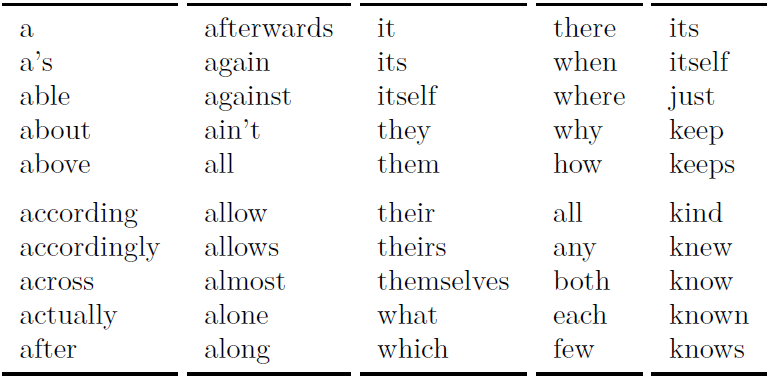
\includegraphics[scale = 0.50]{figuras/stopwords.PNG}
	\fonte{Elaboração do autor.}
\end{table}

Para cada documento de corpo textual das atas do Copom, foi aplicado o processo de \textit{stopwords} (remoção de palavras comuns), provenientes de uma compilação presente no pacote \textit{tidytext} reunido por \citeonline{silge2016tidytext}, que contém 1149 palavras de três diferentes dicionários léxicos: \textit{SMART}, \textit{snowball} e \textit{onix}. Para fins de exemplificação, algumas dessas \textit{stopwords} podem ser observadas na Tabela \ref{table:stopwords}.

Não obstante, palavras adicionais que para a análise desta pesquisa julgou-se irrelevante foram desconsideradas, tais quais meses do ano (como \textit{'january'}, \textit{'month'}, \textit{'monthly'}), nomes próprios (como \textit{'aloisio'}, \textit{'guardado'}, \textit{'rumenos'}), numerais (como \textit{'one'}, \textit{'two'}, \textit{'three'}). Também desconsiderou-se palavras com erros de interpretação devido a quebras de linha (como \textit{'nmonetary'}, \textit{'nexecutive'}, \textit{'npandemic'}).

\subsection{Variáveis macroeconômicas}

Os dados macroeconômicos utilizados para comparação do índice de sentimentos foram reunidos do BCB e do Instituto Brasileiro de Geografia e Estatística (IBGE).

Conforme inicialmente propõe \citeonline{bloom2009uncertainty} e posteriormente \citeonline{ferreira2017incerteza} para o Brasil, baseando-se nesses estudos e considerando algumas alterações, o trabalho englobou as seguintes variáveis:

\begin{enumerate}[noitemsep,nosep,labelindent=\parindent,leftmargin=*,label={\alph*}) ] 
	\item para representar a taxa básica de juros da economia brasileira, usou-se taxa Selic Meta, definida nas reuniões do Copom a cada quarenta e cinco dias;
	\item para a medida de inflação, o Índice Nacional de Preços ao Consumidor Amplo (IPCA), que contempla uma cesta de bens e serviços referentes ao consumo pessoal das famílias de um até quarenta salários mínimos das principais regiões metropolitanas do país;
	\item para a atividade econômica, usou-se do Índice de Atividade Econômica do Banco Central (IBC-Br), que serve como indicador agregado de atividade econômica com frequência mensal;
	\item para representar a produção industrial, utilizou-se a Pesquisa Industrial Mensal de Produção Física (PIM-PF)
\end{enumerate}

A relação resumida das variáveis, sua descrição, seu código nas bases de dados oficiais e sua fonte podem ser observadas na Tabela \ref{table:variaveis_metodologia}:

\begin{table}[hbtp]
	\centering
	\caption{Resumo das variáveis macroeconômicas} \label{table:variaveis_metodologia}
	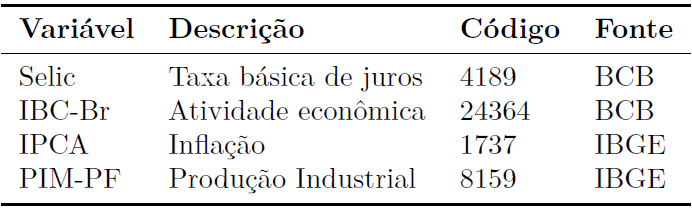
\includegraphics[scale = 0.50]{figuras/variaveis_metodologia.PNG}
	\fonte{Elaboração do autor.}
\end{table}

Os dados de taxa de juros e atividade econômica foram obtidos pelo do Sistema Gerenciador de Séries Temporais (SGS) do BCB, sendo a de código 4189 a taxa de juros Selic acumulada no mês, anualizada base 252, como \%a.a., com periodicidade mensal; e a de código 24364 o "Índice de Atividade Econômica do Banco Central (IBC-Br), aplicado ajuste sazonal, com periodicidade mensal. 

Os dados de inflação e produção industrial foram adquiridos do Sistema IBGE de Recuperação Automática (SIDRA), com código 1737 e 8159, respectivamente.

Como a taxa básica de juros estava anualizada com periodicidade mensal, transformou-se ela em mensal e acumulou-se em número-índice. Da inflação e da taxa básica de juros então calculou-se o valor acumulado em doze meses, de acordo:

\begin{ceqn}
\begin{align} \label{}
\textit{Índice}_{12m, t} = \frac{\textit{Índice}_{t}}{\textit{Índice}_{t-12}} - 1 
\end{align}
\end{ceqn} em que o $\textit{Índice}_{t}$ é o valor do Índice no tempo $t$; o $\textit{Índice}_{t-12}$ é o valor do Índice doze meses após $t$; e $\textit{Índice}_{12m, t}$ é o Índice acumulado no tempo $t$. Com isso, foi possível obter a série da taxa de juros real, descontando a inflação da taxa básica de juros.

Para as séries da inflação e taxa básica de juros haviam-se dados até maio de 2022; para a série da produção industrial até abril de 2022 e para a série de atividade econômica até fevereiro de 2022. Dessa maneira, optou-se por trabalhar com dados até fevereiro de 2022.
% resultados

\chapter{Resultados}

Nesta parte serão apresentados os resultados obtidos através da abordagem metodológica abordada anteriormente. Na Seção \ref{section:estat_desc} são abordadas estatísticas descritivas acerca das atas do Copom. Já na Seção \ref{section:indice_sentimentos} é abordado o índice de sentimentos criado e comparação dele com as variáveis macroeconômicas presentes neste trabalho. Na Seção \ref{section:testes_estac} são expostos os resultados dos testes de estacionariedade para as variáveis macroeconômicas e para o índice. Por fim, a Seção \ref{section:VAR} trata da modelagem econométrica, onde por meio da aplicação de VAR, obtém-se as IRF.

\section{Estatísticas descritivas} \label{section:estat_desc}

Com os dados limpos e tratados, algumas observações iniciais podem ser apontadas. Conforme demonstra-se na Figura \ref{figure:total_words}, no período de Henrique Meirelles na presidência do BCB, tivemos o ápice (4027 palavras) em uma ata do Copom, filtrada por \textit{stopwords}. Outro ponto de destaque é a mudança de média de palavras por ata em três períodos específicos, sendo que o primeiro contempla as atas de número 116 até a de número 180 (média de 3444 palavras por ata), o segundo contempla as atas 181 até 199 (média de 1715 palavras por ata) e o terceiro período as atas de 200 até 246 (média de 1027 palavras por ata).

\begin{figure}[hbtp]
	\centering
	\caption{Número total de palavras por ata, filtrado por \textit{stopwords}} \label{figure:total_words}
	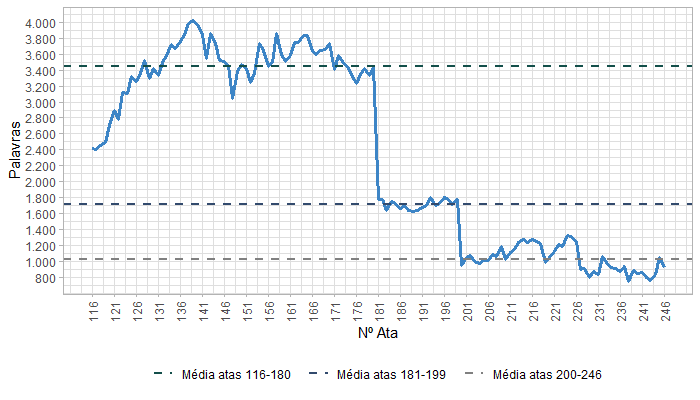
\includegraphics[scale = 0.75]{figuras/grafico_total_words.png}
	\fonte{Elaboração do autor.}
\end{figure}

A alteração do tamanho a partir da ata 181 veio por retirada relevante de seções nos comunicados, onde o cargo de presidência do BCB estava ocupado por Alexandre Tombini. Por fim, a última quebra é referente a ata de número 200 em diante, onde a presidência do BCB se encontrava sob o comando de Ilan Goldfajn, em que houveram mudanças significativas nas estruturas e seções dos comunicados. Vale ressaltar que a quantidade de palavras nas atas do Copom não necessariamente está relacionado a maior qualidade das informações. Neste caso, a redução dos comunicados temporalmente é, em definitivo, uma questão interessante de ser abordada, ainda mais quando o tocante é legibilidade, transparência e credibilidade (maiores detalhes abordados em \citeonline{Omotosho2019}).

Outra questão interessante que merece atenção é em relação as palavras mais frequentes (absolutamente falando) nas atas do Copom em todo o período analisado, conforme a Figura \ref{figure:wordcloud} apresenta, sendo que quanto maior a disposição da palavra, mais frequentemente ela é observada. 

De antemão, destaca-se termos como \textit{'inflation'}, \textit{'prices'}, \textit{'rate'}, \textit{'monetary + policy'}, \textit{'market + expectations'}, entre outras palavras relevantes. Vale notar-se também a alta correlação de $0,81$ entre os termos \textit{'inflation'} e \textit{'increased'}, denotando um alto aparecimento conjunto dessas palavras, isto é, aumento da inflação é um tópico muito recorrente nas atas do Copom, conforme o esperado.

Tais palavras estão em consonância com os objetivos tanto principais como secundários de um Banco Central, isto é, foco na estabilidade de preços, nível de atividade econômica e sinais acerca de políticas posteriores, fornecendo expectativas ao mercado \cite{blinder2000central, mishkin2000, bernanke2004monetary}.

\begin{figure}[hbtp]
	\centering
	\caption{Núvem de palavras mais frequentes nas atas} \label{figure:wordcloud}
	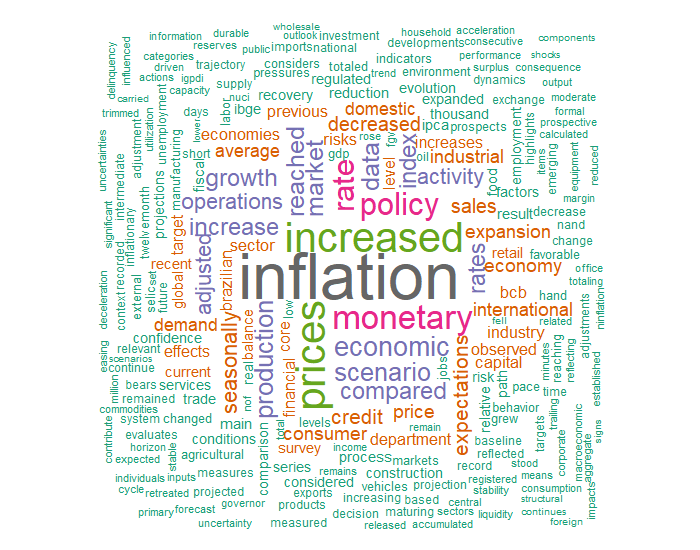
\includegraphics[scale = 0.75]{figuras/wordcloud_copom_words.png}
	\fonte{Elaboração do autor.}
\end{figure}

Após ter-se visualizado de forma ampla os termos mais recorrentes englobando todas as atas desde janeiro de 2006 até maio de 2022, separou-se as palavras que mais apareceram em cada ata. Como por exemplo, conforme observado na Figura \ref{figure:absolut_freq_words}, tem-se as oito palavras mais frequentes de uma sub-amostra, da ata 235 até a ata 246. Tal qual o esperado e apontado anteriormente pela Figura \ref{figure:wordcloud}, \textit{'inflation'} é o termo que aparece como mais corriqueiro para todas as atas, confirmado pelas atas da sub-amostra. Termos como \textit{'monetary'}, \textit{'scenario'}, \textit{'policy'}, \textit{'economic'} e \textit{'rate'} também são homogeneamente comuns. Detalhe para o surgimento no pódio entre as oito mais citadas da palavra \textit{'risks'} na ata 236 até a ata 242, saindo e reaparecendo na ata 246.

\begin{figure}
	\centering
	\caption{Palavras mais frequentes nas atas do Copom (atas nº 235 até nº 246)} \label{figure:absolut_freq_words}
	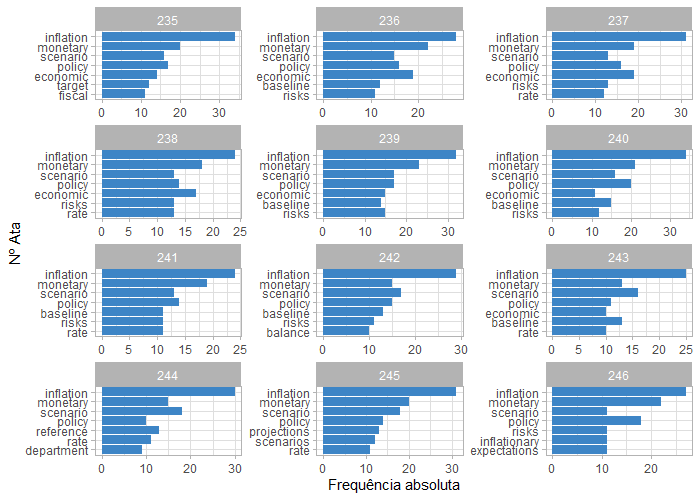
\includegraphics[scale = 0.75]{figuras/words_frequency_copom_text.png}
	\fonte{Elaboração do autor.}
\end{figure}

De qualquer maneira, apesar de ser interessante a reafirmação dos termos discutidos nas atas em relação aos objetivos de um comunicado de fonte oficial desta grandeza, pode-se constatar que em linhas gerais as palavras se repetem muito. Uma maneira de contornar essa questão e tentar extrair as palavras com maior importância de cada ata, é tornar a atenção para as frequências dos termos (\textit{tf}) em relação à frequência inversa do documento (\textit{idf}), denominada estatística tf-idf, abordada anteriormente na seção metodológica.

Como enunciado em \citeonline{silge2017text}, a parte \textit{idf} desta relação de frequências diminui o peso para palavras que aparecem muitas vezes nos documentos e aumenta o peso para palavras que não aparecem muitas vezes, sendo que uma vez multiplicado pela parte \textit{tf} nos resulta na frequência do termo ajustado por quão raramente ele aparece nos comunicados, isto é, extrai-se as palavras mais relevantes para cada ata dentro do período de análise proposto.

\begin{figure}
	\centering
	\caption{Frequências relativas, visualização das caudas longas (atas nº 238 até nº 246)} \label{figure:relative_freq_histograms}
	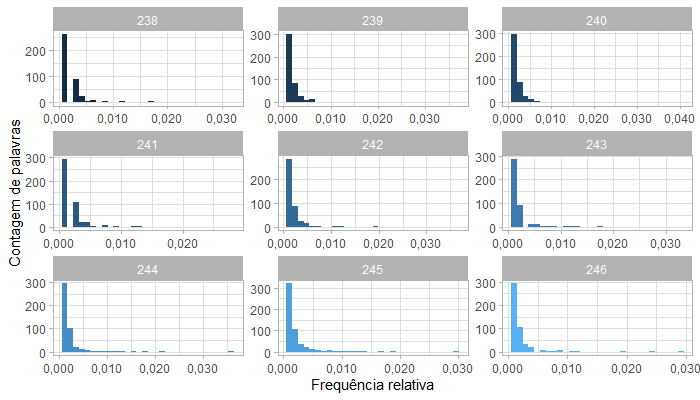
\includegraphics[scale = 0.75]{figuras/histogram_freq_words.png}
	\fonte{Elaboração do autor.}
\end{figure}

Mediante demonstrado pelos histogramas na Figura \ref{figure:relative_freq_histograms}, por meio da frequência relativa (número de vezes que determinada palavra aparece em determinada ata dividido pelo número de palavras naquela ata) pode-se perceber que existem muitos termos nas caudas da distribuição (que aparecem poucas vezes), sendo assim, poucas palavras que aparecem muitas vezes e muitas palavras que aparecem poucas vezes.

Salienta-se que distribuições de cauda longa como as representadas na Figura \ref{figure:relative_freq_histograms}, são comuns no estudo estatístico-linguístico dado um \textit{Corpus} (neste caso os documentos das atas do Copom), onde há uma relação inversamente proporcional entre a frequência em que determinada palavra aparece e o rank (ordenação da maior para menor frequência) dessa mesma palavra. A versão clássica dessa relação é chamada Lei de Zipf \cite{piantadosi2014zipf}.

\begin{table}[hbtp]
	\centering
	\caption{Estatísticas \textit{tf-idf} para palavras da ata nº 246} \label{table:tf_idf}
	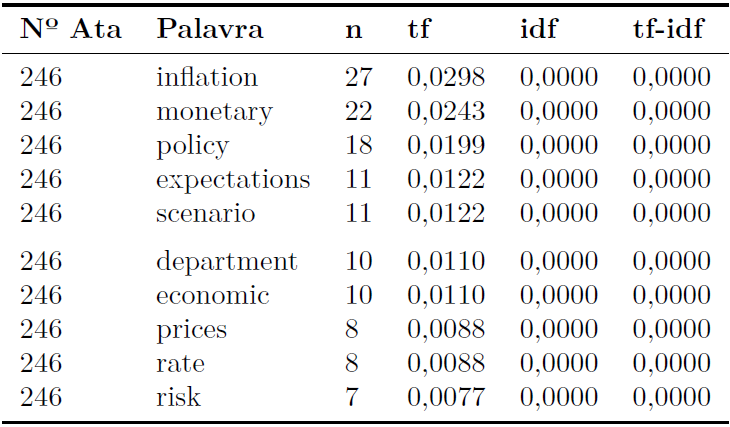
\includegraphics[scale = 0.50]{figuras/tabela_tf_idf.PNG}
	\fonte{Elaboração do autor.}
\end{table}

Tomando a ata nº 246 como exemplo, conforme apresentado na Tabela \ref{table:tf_idf}, tem-se a palavra, a quantidade de vezes que ela aparece na determinada ata, a frequência do termo (\textit{tf}), frequência inversa do documento (\textit{idf}) e a estatística \textit{tf-idf}. Como é possível contemplar, para palavras que são muito comuns entre todas as atas (\textit{'inflation'}, \textit{'expectations'}, \textit{'prices'} etc.), a \textit{idf} será zero (e por consequência a estatística \textit{tf-idf} também), uma vez que $\ln(1) = 0 $.

Já, quando olha-se para as maiores estatísticas \textit{tf-idf}, por exemplo, da ata nº 227 até a ata nº 246, consoante a Figura \ref{figure:tf_idf}, tem-se resultados muito promissores e interessantes. Primeiramente, percebe-se de forma notória que as palavras se diferem bastante entre si e em relação àquelas presentes na Figura \ref{figure:absolut_freq_words}. 

\begin{figure}[hbtp]
	\centering
	\caption{Estatísticas \textit{tf-idf} (atas nº 227 até nº 246)} \label{figure:tf_idf}
	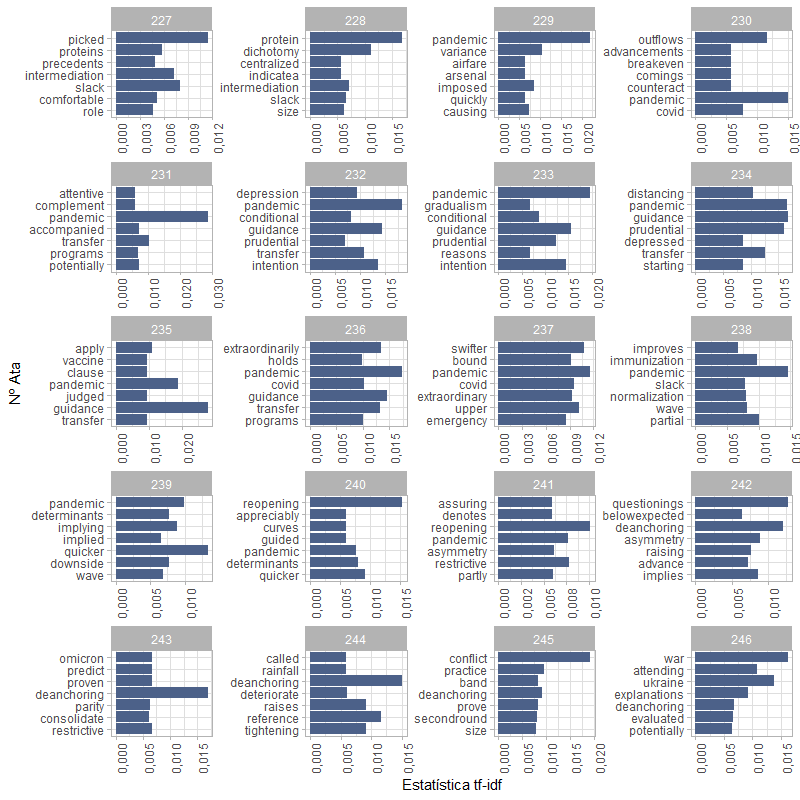
\includegraphics[scale = 0.75]{figuras/tf_idf_copom_text_refined.png}
	\fonte{Elaboração do autor.}
\end{figure}

Além disso, se nota não só o surgimento da palavra \textit{'pandemic'} a partir da ata nº 229, como sua persistência até a ata 240, com alta relevância. Na ata nº 229, pode-se perceber o aparecimento da palavra \textit{'airfare'} (referente à variação nos preços de passagens aéreas devido à retração do preço internacional do barril de petróleo), assim como a palavra \textit{'imposed'}, em relação às restrições impostas; ambas referências como consequência do estourar da pandemia do Coronavírus em 2020. 

Na ata nº 230, tem-se o surgimento da palavra \textit{'outflows'}, referente a fortes saídas de capital no Brasil (um país emergente) em momentos incertos e de alto risco financeiro. Também rassalta-se o surgimento de \textit{'transfer + programs'} na ata nº 231, acerca da implementação de programas de crédito e transferência de renda a famílias vulneráveis. No intermédio, destacam-se termos como \textit{'prudential'}, \textit{'gradualism'}, \textit{'distancing'}, \textit{'vaccine'}, \textit{'emergency'}, \textit{'immunization'}, \textit{'partial + normalization'}, \textit{'restrictive'}, \textit{'omicron'}, todos relacionados à crise sanitária. 

Outrossim, observa-se na ata 240, a inauguração do termo \textit{'reopening'} em alusão ao início da reabertura da economia como um todo. Atenta-se também para o surgimento de \textit{'deanchoring'} na ata nº 242 (perdurando até a 246), tratando-se da desancoragem das expectativas de inflação. Por fim, tem-se termos como \textit{'conflict'} e \textit{'ukraine'} devido à invasão da Ucrânia por parte da Rússia, iniciada em fevereiro de 2022.

Feitas análises de estatísticas descritivas referente ao período proposto, categorizou-se as palavras presentes nos documentos em positivas ou negativas e criou-se um índice de sentimentos das atas do Copom.

\section{Índice de sentimentos das Atas do Copom} \label{section:indice_sentimentos}

No presente trabalho, foi utilizado o dicionário léxico proposto por \citeonline{bing_liu_2004}, que conta com 6.786 palavras classificadas com teor positivo ou negativo, onde alguns desses termos podem ser observados na Tabela \ref{table:bing_liu}. É importante destacar que esse método desconsidera bigramas (\textit{'no good'}, \textit{'not true'}, \textit{'no risks'}, \textit{'no volatility'}), ou seja, ele é baseado somente em unigramas, que são palavras isoladas \cite{silge2017text}.

\begin{table}[hbtp]
	\centering
	\caption{Palavras presentes no dicionário de sentimentos proposto por \citeonline{bing_liu_2004}} \label{table:bing_liu}
	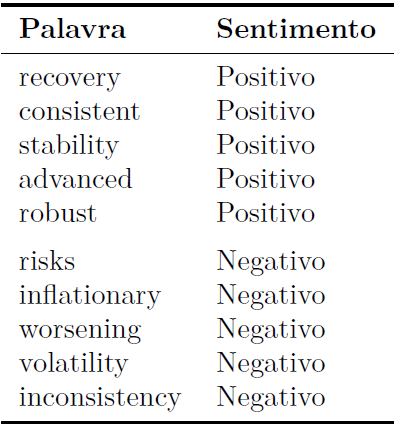
\includegraphics[scale = 0.50]{figuras/palavras_hu_liu2004.PNG}
	\fonte{Elaboração do autor.}
\end{table}

Cruzando as informações das atas do Copom que foram adquiridas por meio da raspagem de dados \textit{web} e posteriormente tratadas, com as informações presentes no dicionário léxico, encontrou-se o número de palavras categorizadas como positivas e negativas para cada documento de texto. 

\begin{table}[hbtp]
	\centering
	\caption{Sentimentos encontrados nas atas do Copom} \label{table:sentiment_index}
	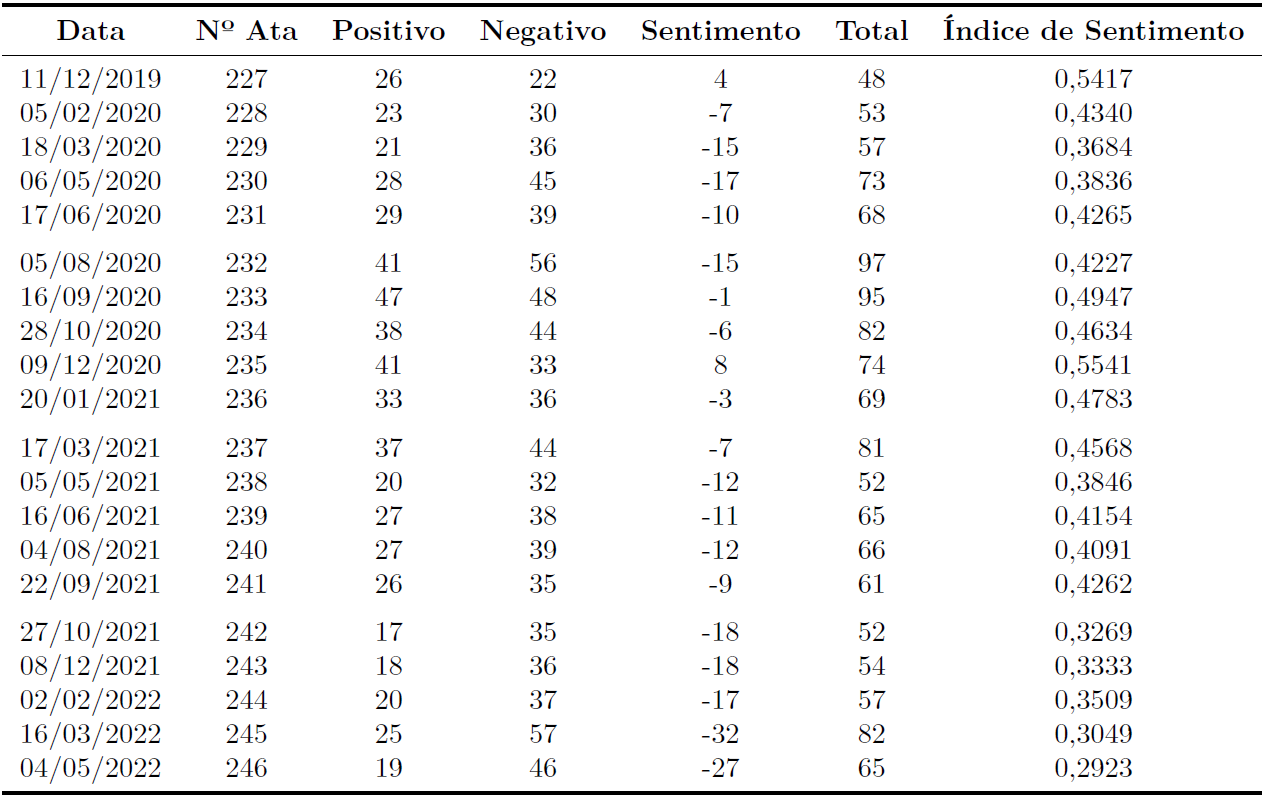
\includegraphics[scale = 0.45]{figuras/tabela_sentimento.PNG}
	\fonte{Elaboração do autor.}
\end{table}

Pós cruzamento dos dados e categorização das palavras, se baseando em \citeonline{bholat_etal2015}, criou-se o índice de sentimentos a seguir:

\begin{ceqn}
\begin{align} \label{eq:eq_sentiment_index}
 IS_{t} = \frac{NP_{t}}{NP_{t} - NN_{t}} 
\end{align}
\end{ceqn} onde, na equação \eqref{eq:eq_sentiment_index}, tem-se que $IS_{t}$ é o índice de sentimento para a ata no tempo $t$; $NP_{t}$ é a quantidade de palavras categorizadas como positivas para a ata no tempo $t$; e $NN_{t}$ é a quantidade de palavras categorizadas como negativas para a ata no tempo $t$.

Sendo assim, como $0 \leq IS_{t} \leq 1$, quando o valor for acima de $0,5$ tem-se uma perspectiva otimista para a economia, caso contrário, temos a definição do sentimento de pessimismo. Destaca-se também que quanto mais próximo de $1$ o valor, mais otimista a ata, assim como quanto mais próximo de $0$, mais pessimista.

Para exemplificar, na Tabela \ref{table:sentiment_index}, estão dispostas informações do índice de sentimentos criado, da ata nº 227 até a de nº 246. A coluna \textit{Positivo} é o $NP_{t}$, a coluna \textit{Negativo} o $NN_{t}$, a coluna \textit{Sentimento} é o saldo (positivas subtraídas das negativas), a coluna \textit{Total} é a soma das palavras categorizadas e a última coluna é referente ao índice. Como é possível observar, das atas presentes na tabela, somente a 227 e 235 tiveram um saldo tido como otimista (e com baixo grau, de $0,5417$ e $0,5541$ respectivamente), o restante teve um teor negativo, com destaque para a ata nº 246 com um $IS_{246} = 0,2923$. 

\begin{figure}[hbtp]
	\centering
	\caption{Índice de sentimento das atas do Copom} \label{figure:sentiment_index}
	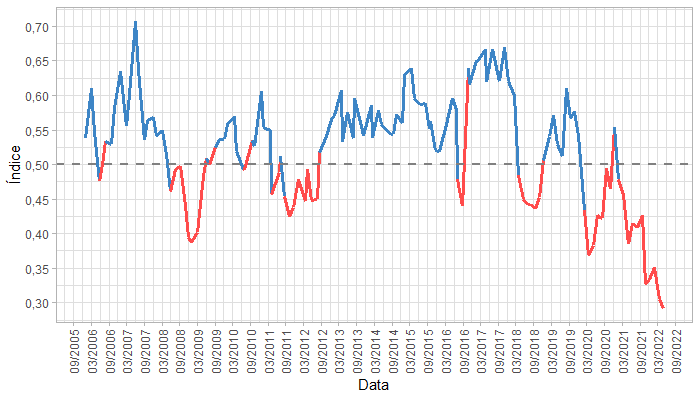
\includegraphics[scale = 0.75]{figuras/indice_de_sentimentos.png}
	\fonte{Elaboração do autor.}
\end{figure}

Por fim, foi elaborado um gráfico, conforme a Figura \ref{figure:sentiment_index}, com a série temporal do $IS_{t}$ criado, em que $t = 116,...,246$. A coloração da linha em azul representa períodos com um $IS_{t} > 0,5$ e a coloração em vermelho, um $IS_{t} \leq 0,5$. Na maior parte do tempo (82 das atas), observa-se o índice indicando teor positivo, enquanto no restante, inclusive para o período mais recente, nota-se o teor negativo (49 das atas).

Chega-se na conclusão de que, de forma geral, o Copom aborda seus comunicados acerca da condução de política monetária e assuntos relacionados à atividade e conjuntura econômica no Brasil de maneira otimista. Com o índice elaborado, comparou-se ele com variáveis macroeconômicas de interesse.

\subsection{Comparando o índice com variáveis macroeconômicas}

Assim como nos exercícios realizados por \citeonline{bloom2009uncertainty} e \citeonline{ferreira2017incerteza}, para as séries do Índice de Sentimentos, IBC-Br e PIM-PF foram extraídos os componentes cícliclos por meio do filtro de \citeonline{hp_filter1997}.

\begin{figure}[hbtp]
	\centering
	\caption{Séries macroecônomicas pós-tratamento} \label{figure:series_macro}
	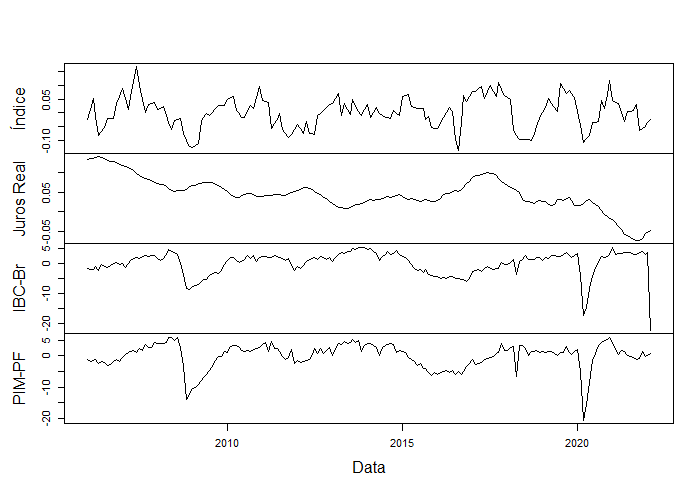
\includegraphics[scale = 0.75]{figuras/graf_series_macro.png}
	\fonte{Elaboração do autor.}
\end{figure}

A Figura \ref{figure:series_macro} demonstra as séries temporais das quatro variáveis que posteriormente serão inclusas no modelo VAR. Atenta-se para o fato de que o índice de sentimentos criado aparenta acompanhar as demais variáveis selecionadas em momentos críticos na economia, como, por exemplo, em 2008 com a Crise Financeira do Subprime e em 2020 com a Crise Sanitária do Covid-19. Além disso, é possível observar uma tendência de queda da taxa de juros real em nível, enquanto as demais séries aparentam ser estáveis.

\section{Resultados dos testes de estacionariedade} \label{section:testes_estac}

Conforme mencionado anteriormente, as variáveis inclusas em modelos VAR($p$) precisam possuir a característica de estacionariedade. Dessa maneira, foram realizados testes de raiz unitária de Dickey-Fuller (DF) e Dickey-Fuller Aumentado (ADF) - com uma defasagem - e de Kwiatkowski–Phillips–Schmidt–Shin (KPSS). 

\begin{table}[hbtp]
	\centering
	\caption{Resultados dos testes ADF sem constante e sem tendência} \label{table:adf_none}
	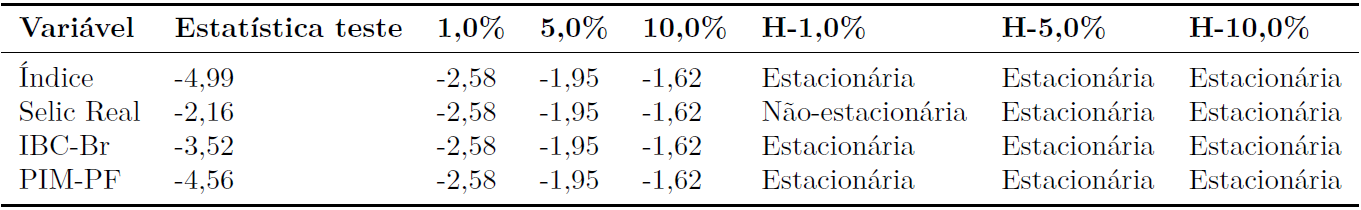
\includegraphics[scale = 0.40]{figuras/teste_adf_none.PNG}
	\fonte{Elaboração do autor.}
\end{table}

Primeiramente, conforme observa-se na Tabela \ref{table:adf_none}, elaborou-se o teste de ADF sem constante e sem tendência. A primeira e segunda coluna representam a variável e sua respectiva estatística do teste; já as colunas "$1,0\%$", "$5,0\%$" e "$10,0\%$" representam os níveis de significância ($\alpha$); e por fim as colunas "H-$1,0\%$", "H-$5,0\%$" e "H-$10,0\%$" indicam se a série é estacionária ou não através da aceitação ou não da hipótese nula. 

Por meio deste teste constata-se que praticamente todas as séries rejeitam a hipótese nula ($H_{0}$) de não-estacionariedade, portanto são estacionárias para todos os níveis de significância propostos, exceto para a série dos juros reais a um $\alpha = 1,0\%$.

\begin{table}[hbtp]
	\centering
	\caption{Resultados dos testes ADF com constante} \label{table:adf_drift}
	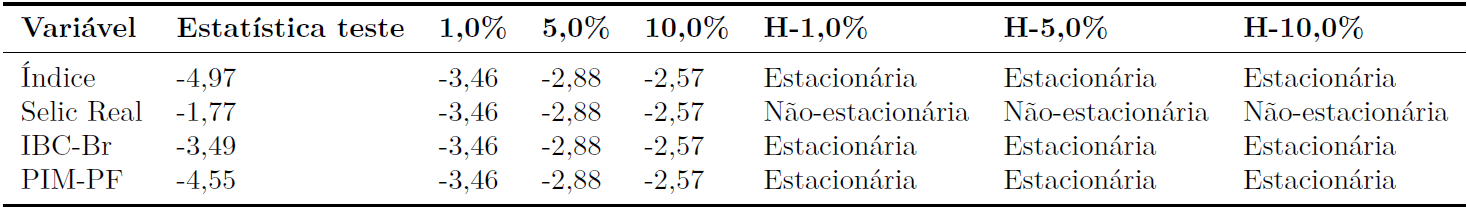
\includegraphics[scale = 0.40]{figuras/teste_adf_drift.PNG}
	\fonte{Elaboração do autor.}
\end{table}

Quando feito o teste de ADF com constante, conforme a Tabela \ref{table:adf_drift} demonstra, a série dos juros reais não só é tida como não-estacionária a um $\alpha = 10,0\%$, mas como para $\alpha = 5,0\%$ e $\alpha = 1,0\%$ também.

Elaborando o teste de ADF com constante e tendência, como contempla-se na Tabela \ref{table:adf_trend}, além das taxas de juros reais não serem estacionárias, tem-se que para níveis de significância de $5,0\%$ e $1,0\%$, o IBC-Br também apresenta não-estacionariedade.

\begin{table}[hbtp]
	\centering
	\caption{Resultados dos testes ADF com constante e com tendência} \label{table:adf_trend}
	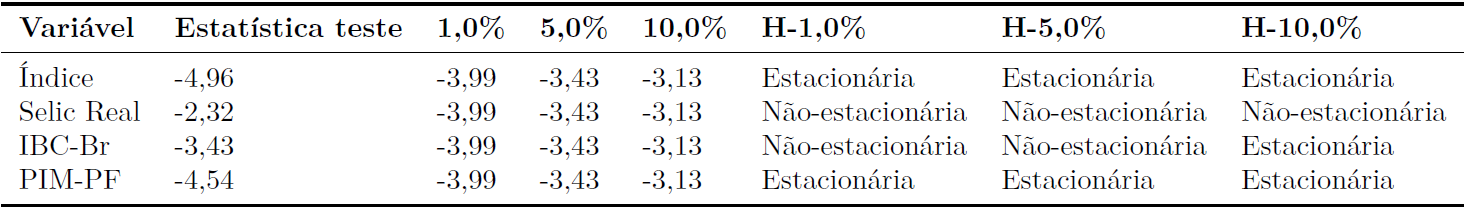
\includegraphics[scale = 0.40]{figuras/teste_adf_trend.PNG}
	\fonte{Elaboração do autor.}
\end{table}

Por fim, por meio do teste de KPSS, em que a hipótese nula ($H_{0}$) é a de estacionariedade, tem-se que somente a série das taxas de juros reais rejeita $H_{0}$, conforme está disposto na Tabela \ref{table:kpss}.

\begin{table}[hbtp]
	\centering
	\caption{Resultados dos testes KPSS} \label{table:kpss}
	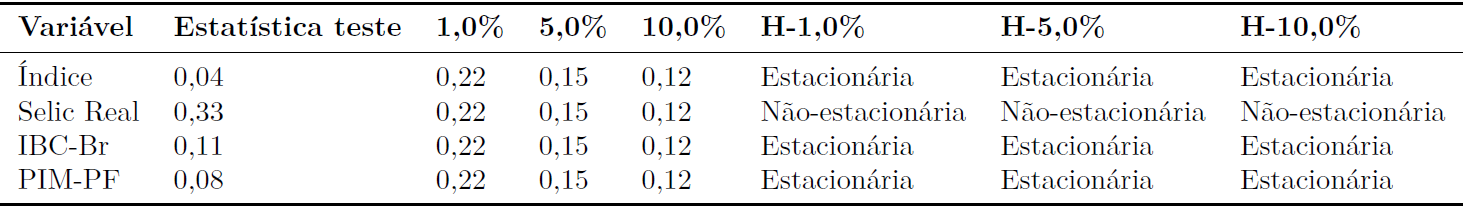
\includegraphics[scale = 0.40]{figuras/teste_kpss.PNG}
	\fonte{Elaboração do autor.}
\end{table}

\pagebreak{}

Desta maneira, optou-se por manter todas as séries em seus níveis, exceto para a série dos juros reais, em que foi feita uma diferenciação, como pode ser observado na Figura \ref{figure:series_macro_2}.

\begin{figure}[hbtp]
	\centering
	\caption{Séries macroeconômicas pós-tratamento, com juros real diferenciado} \label{figure:series_macro_2}
	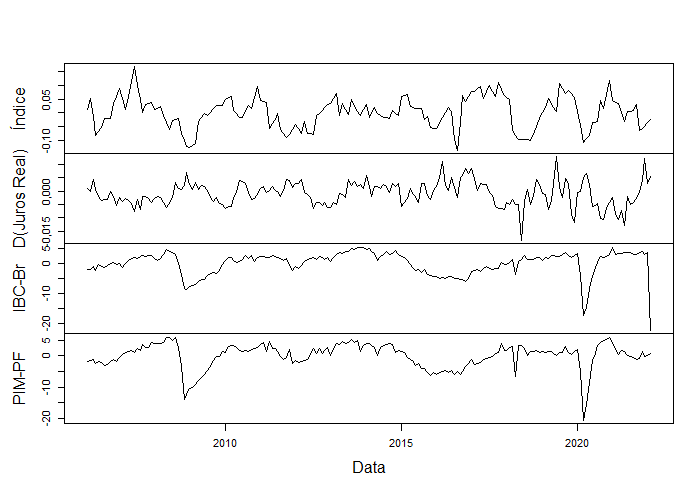
\includegraphics[scale = 0.75]{figuras/graf_series_macro_2.png}
	\fonte{Elaboração do autor.}
\end{figure}

Após isso, todos os testes foram refeitos e para um $\alpha = 5,0\%$, que é o nível de significância desejado, constatou-se que todas as séries são estacionárias, prontas para serem inclusas no modelo VAR.

%\subsection{Dickey-Fuller Aumentado (ADF)}

%\subsection{Phillips-Perron (PP)}

%\subsection{Kwiatkowski–Phillips–Schmidt–Shin (KPSS)}

%\section{Resultados dos testes de cointegração}

%\section{Resultados do mecanismo de correção de erros (MCE)}

\section{Resultados do modelo de vetores autorregressivos (VAR)} \label{section:VAR}

Detendo o conjunto de variáveis estacionárias, a estimação do modelo VAR($p$) pode ser efetuada, onde os critérios de decisão abordados nas Equações \eqref{eq:BIC}, \eqref{eq:AIC} e \eqref{eq:HQ} são utilizados para se definir as ordens ótimas de defasagens. Após isso, visto que a estabilidade do modelo e de seus parâmetros foram garantidas, foi selecionada a ordem que apresentou os melhores testes de diagnóstico.

A partir dos critérios $BIC(p,q)$ e $HQ(p,q)$ o número de defasagens ótimo apontado foi de 1, enquanto para o critério $AIC(p,q)$ o número aumenta para 2. Dessa forma, foram estimados dois modelos, contemplando as duas possibilidades de defasagens propostas pelos critérios de informação. Tanto para uma quanto para duas defasagens, as raízes do polinômio característico ficaram abaixo de um, ou seja, fora do círculo unitário, além dos testes de flutuação empírica, abordado em \citeonline{ploberger1992cusum}, evidenciarem parâmetros estáveis, isto é, sem quebras estruturais (os resultados podem ser constatados no Apêndice A).

%No modelo de VAR($1$), para a equação do índice de sentimentos o coeficiente de determinação ajustado foi de $R_{adj}^2 = 0,659$; enquanto que para a equação da taxa de juros real diferenciada, o $R_{adj}^2 = 0,416$. Para a equação da atividade econômica, obteve-se um $R_{adj}^2 = 0,623$; ao passo que a equação da produção industrial resultou num $R_{adj}^2 = 0,697$, sendo o maior entre todos. 

Para o modelo VAR($1$), o teste conjunto de autocorrelação serial de Breusch-Godfrey falhou, dado que o p-valor = $0,007$, abaixo de p-valor = $0,05$. Considerando os testes individuais, somente a série do D(Juros Real) e a série do IBC-Br entregaram um p-valor > $0,05$. Enquanto, para o teste conjunto ARCH de heterocedasticidade, o modelo apresentou estar estável, já que retornou um p-valor = $0,10$.

Dessa maneira, optou-se trabalhar com o VAR($2$), onde o teste conjunto de autocorrelação serial de Breusch-Godfrey apresentou como p-valor = $0,10$, acima de p-valor = $0,05$, denotando assim que não há autocorrelação nos resíduos das séries do modelo estimado. Considerando os testes individuais, todas as séries apresentaram um p-valor > $0,05$, isto é, individualmente também não apresentam correlação serial. Enquanto que, para o teste conjunto ARCH de heterocedasticidade, o modelo apresentou estar estável, retornando um p-valor = $0,10$.

No VAR($2$), considerando todas as variáveis como endógenas, obteve-se então o seguinte sistema de equações:

\begin{ceqn}
\begin{align} \label{eq:sist_equacoes_var_2}
&IS_{t} = IS_{t-1} + \Delta JR_{t-1} + AE_{t-1} + PI_{t-1} + IS_{t-2} + \Delta JR_{t-2} + AE_{t-2} + PI_{t-2} + \epsilon_{IS_{t}} \\
&\Delta JR_{t} = IS_{t-1} + \Delta JR_{t-1} + AE_{t-1} + PI_{t-1} + IS_{t-2} + \Delta JR_{t-2} + AE_{t-2} + PI_{t-2} + \epsilon_{\Delta JR_{t}} \\
&AE_{t} = IS_{t-1} + \Delta JR_{t-1} + AE_{t-1} + PI_{t-1} + IS_{t-2} + \Delta JR_{t-2} + AE_{t-2} + PI_{t-2} + \epsilon_{AE_{t}} \\
&PI_{t} = IS_{t-1} + \Delta JR_{t-1} + AE_{t-1} + PI_{t-1} + IS_{t-2} + \Delta JR_{t-2} + AE_{t-2} + PI_{t-2} + \epsilon_{PI_{t}}
\end{align}
\end{ceqn} onde a equação do índice de sentimentos ($IS$) chegou a um coeficiente de determinação ajustado no valor de $R_{adj}^2 = 0,667$; ao passo que para a equação da taxa de juros real diferenciada ($\Delta JR$), o $R_{adj}^2 = 0,429$. Para a equação da atividade econômica ($AE$), resultou-se num $R_{adj}^2 = 0,626$; enquanto a equação da produção industrial ($PI$) decorreu em um $R_{adj}^2 = 0,722$, sendo o maior entre todos. Os coeficientes das equações podem ser vistos no Apêndice A.

\subsection{Causalidade de Granger}

%Para o modelo de VAR($1$), nos testes individuais de causalidade de Granger, nenhuma variável apresentou Granger-causar o índice de sentimentos criado para um nível de $\alpha = 5,0\%$. No sentido do índice Granger-causar as variáveis, apenas a atividade econômica e a produção industrial apresentaram rejeição à $H_{0}$ de não-causalidade, porém apenas para um $\alpha = 10,0\%$. Entretanto, para o teste conjunto de causalidade tem-se para todas as variáveis um p-valor > $0,05$, dessa forma rejeitando a hipótese nula de não-causalidade, ou seja, todas as variáveis Granger-causam o índice de sentimentos.

No modelo VAR($2$), para os testes individuais de causalidade de Granger, nenhuma variável apresentou Granger-causar o índice de sentimentos criado para um nível de $\alpha = 5,0\%$. Considerando o índice Granger-causar as variáveis, conforme observa-se na Tabela \ref{table:granger_individual_model2}, tem-se que apenas a PIM-PF é afetada, para um $\alpha = 5,0\%$, sendo seu p-valor = $0,02$.

\begin{table}[hbtp]
	\centering
	\caption{Testes individuais de causalidade de Engle-Granger para o VAR($2$)} \label{table:granger_individual_model2}
	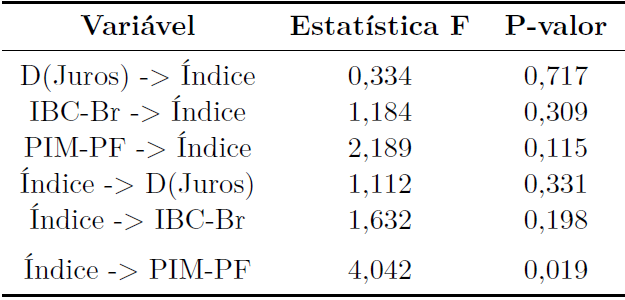
\includegraphics[scale = 0.45]{figuras/granger_individual_model2.PNG}
	\fonte{Elaboração do autor.}
\end{table}

Para o teste em conjunto de causalidade de Granger, como apresentado na Tabela \ref{table:granger_conjunto_model2}, tem-se um p-valor > $0,05$ para as variáveis da diferença da taxa de juros real e produção industrial, assim essas variáveis não Granger-causam o índice e as outras variáveis, apesar de que para a atividade econômica o p-valor = $0,04$, fazendo com que o IBC-Br possa Granger-causar o índice criado, tanto quanto as outras variáveis, ou todas, entretanto como visto no teste individual, o IBC-Br não Granger-causa o índice.

\begin{table}[hbtp]
	\centering
	\caption{Teste conjunto de causalidade de Engle-Granger para o VAR($2$)} \label{table:granger_conjunto_model2}
	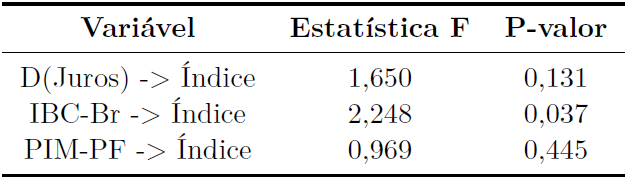
\includegraphics[scale = 0.50]{figuras/granger_conjunto_model2.PNG}
	\fonte{Elaboração do autor.}
\end{table}

\subsection{Funções impulso-resposta (IRF)}

A análise das Funções de Impulso-Resposta demonstrou, conforme a Figura \ref{figure:irf_indice_indice_model_2} aponta que, dado um choque positivo no índice, a resposta do próprio índice sofre positivamente com impacto decrescente, segundo o tamanho do choque dado, de forma significativa. Salienta-se que para o VAR($2$), a partir do 6º período, o choque deixa-se de ser significante para um intervalo de confiança de $95,0\%$.

\begin{figure}[hbtp]
	\centering
	\caption{IRF do VAR($2$): Índice $\rightarrow$ Índice} \label{figure:irf_indice_indice_model_2}
	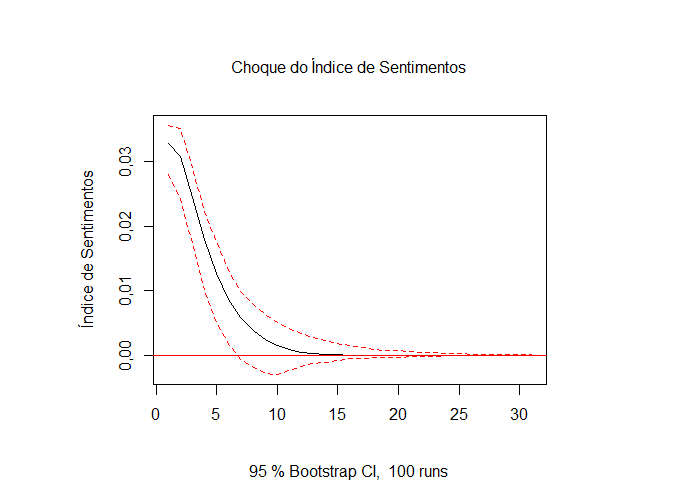
\includegraphics[scale = 0.60]{figuras/irf_indice_indice_model_2.PNG}
	\fonte{Elaboração do autor.}
\end{figure}


Já, a partir de um choque efetuado no índice em relação à diferença dos juros reais, como observa-se na Figura \ref{figure:irf_indice_selic_model_2}, tem-se uma resposta negativa até o 4º período (sendo este um ponto de inflexão), aumentado com o passar dos períodos. Entretanto, para o VAR($2$), o choque é somente significativo entre o 4º e 5º período, para $95,0\%$ de confiança.

\begin{figure}[hbtp]
	\centering
	\caption{IRF do VAR($2$): Índice $\rightarrow$ D(Juros)} \label{figure:irf_indice_selic_model_2}
	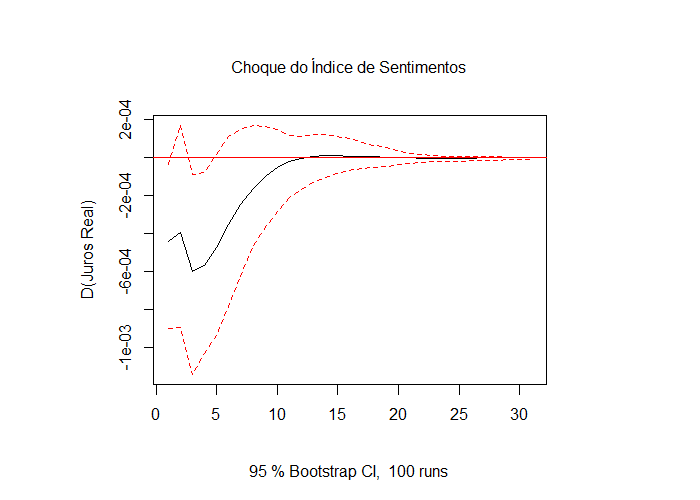
\includegraphics[scale = 0.60]{figuras/irf_indice_selic_model_2.PNG}
	\fonte{Elaboração do autor.}
\end{figure}

Outrossim, quando se atenta à resposta da atividade econômica dado um choque no índice de sentimentos, percebe-se conforme a Figura  \ref{figure:irf_indice_ibcbr_model_2} aponta, que os impactos são sentidos a partir do 2º mês, perdurando significativamente (intervalo de confiança de $95,0\%$) até o 5º período para o VAR($2$). Do choque até o quinto período, tem-se uma reação positiva, sendo que a partir do 5º, ela decai.

\begin{figure}[hbtp]
	\centering
	\caption{IRF do VAR($2$): Índice $\rightarrow$ IBC-Br} \label{figure:irf_indice_ibcbr_model_2}
	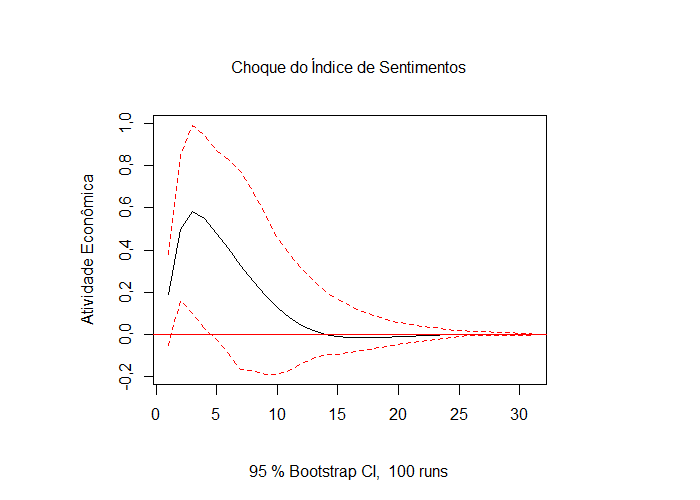
\includegraphics[scale = 0.60]{figuras/irf_indice_ibcbr_model_2.PNG}
	\fonte{Elaboração do autor.}
\end{figure}

Por fim, dado um impulso no índice, a resposta da produção industrial se assemelha com a da atividade econômica, onde como se observa na Figura \ref{figure:irf_indice_pimpf_model_2}, há um pico no 5º período, onde a partir dele, os choques deixam de ser significativos.

\begin{figure}[hbtp]
	\centering
	\caption{IRF do VAR($2$): Índice $\rightarrow$ PIM-PF} \label{figure:irf_indice_pimpf_model_2}
	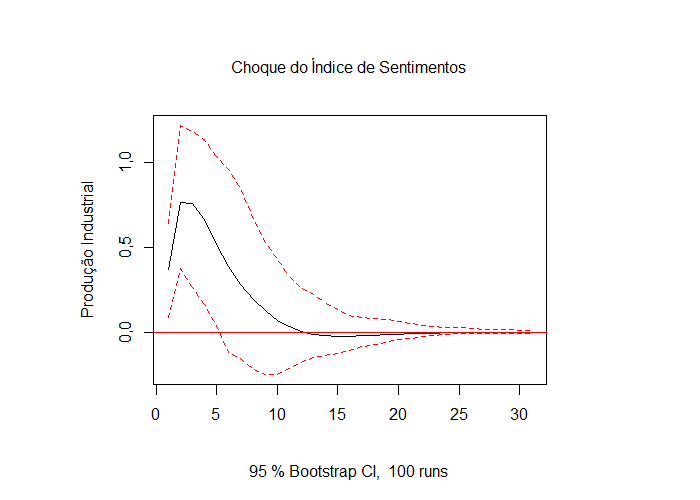
\includegraphics[scale = 0.60]{figuras/irf_indice_pimpf_model_2.PNG}
	\fonte{Elaboração do autor.}
\end{figure}

Em \citeonline{ferreira2017incerteza}, são disponibilizados apenas os resultados das IRF de atividade econômica e produção industrial, dado um choque no IIE-Br, onde ambas respondem negativamente, com pequenos intervalos significantes, semelhantes aos resultados do trabalho de \citeonline{bloom2009uncertainty}. As possíveis divergências com os resultados obtidos neste trabalho, provavelmente se dão, pois, os autores criaram índices de incerteza da economia e não um índice de sentimentos das atas do Copom. Não só isso, os autores contemplaram um número maior de variáveis, como câmbio, desemprego e preços de commodities, além de impor uma restrição de ordenamento das variáveis, o que ia além da proposta deste trabalho. Interessante apontar que, por ainda serem incipientes os estudos que relacionam mineração textual, análise de sentimentos e economia, os resultados podem servir como norteadores de alguma forma.

Dessa maneira, conclui-se que por meio de choques aos sentimentos dos comunicados das atas do Copom, a diferença da taxa de juros básica acumulada em doze meses, descontada da taxa de inflação (também acumulada em doze meses), sofre negativamente, ao qual se estabiliza conforme se avança nos períodos. Entretanto, quando se olha para a atividade econômica e para a produção industrial, percebe-se que a resposta é positiva com impactos decrescentes, também se estabilizando em torno de zero conforme o avanço do tempo, visto que os choques não possuem efeitos permanentes em séries temporais que possuem a característica de estacionariedade. 
% considerações finais

\chapter{Considerações Finais}

Este estudo buscou elucidar sobre a importância da comunicação e transparência de um Banco Central, isto é, toda informação disponibilizada para os agentes externos, que envolve a condução da política monetária, em relação à atividade econômica e em relação à sinais de trajetórias futuras. Foi apontado, que os níveis atuais de comunicação e transparência foi um trajeto percorrido ao longo dos anos, assim como um movimento internacional.

Dessa forma, como ferramenta de comunicação, o BCB se utiliza das atas do Copom, além da abordagem de transparência adotada por meio do RMI. Com isso, quando se fala da relação entre a discrição e regra, de forma rara um Banco Central seguirá rigorosamente as regras, uma vez que tem-se o chamado viés inflacionário, isto é, o impulso de se diminuir o desemprego ou aumentar o produto. Nesse sentido, quando o RMI não possui credibilidade, a tendência é resultar na discrição, aumentando a oferta de moeda e por consequência gerando uma taxa de inflação maior.

Com isso em mente, apresentaram-se estudos que aplicaram na economia, técnicas de mineração textual, que é um processo para organizar e transformar dados textuais disponíveis em documentos e grandes bases de dados, para extrair significados e padrões. Como as atas do Copom são disponibilizadas no site do BCB, o objetivo deste trabalho foi aplicar essas técnicas para extrair as todas as atas lá presentes, filtrar para o período de 2006 até 2022 e, por meio de análise de sentimentos, criar um índice para os comunicados.

A partir da elaboração do índice, comparou-se ele com variáveis macroeconômicas de interesse, e com os devidos testes econométricos feitos para asseguração da consistência dos resultados, aplicou-se modelagem de vetores autorregressivos, podendo assim inferir ou não causalidade de Granger das variáveis, como também a elaboração de funções de impulso-resposta.

Os critérios de informação para escolha do número de defasagens do modelo apontou para uma e duas, entretanto, como o VAR($1$) falhou no teste de autocorrelação serial dos resíduos, trabalhou-se somente com o VAR($2$). Dessa maneira, foi possível sair de uma simples correlação para uma análise de causalidade, onde obteve-se que o índice Granger-causa a produção industrial e as variáveis de taxa de juros real e produção industrial Granger-causam o índice. Analisando as IRF, para os juros reais, tem-se uma resposta negativa, sendo os choques significativos para o 4º e 5º período; para a atividade econômica, os impactos são sentidos no 2º mês, perdurando significativamente até o 5º período; e por fim, a resposta da produção industrial é afetada positivamente, com um pico de impacto no 5º período.

Enfim, reitera-se que este trabalho procurou contribuir com a aplicação da intersecção de técnicas de mineração textual, análise de sentimentos e macroeconomia, além de considerar técnicas estatísticas-econométricas para contribuir com a robustez das resultantes, com o VAR cumprindo o proposto no trabalho. Como trabalhos futuros, pode-se sugerir modelagens preditivas, levando em consideração que o VAR é um ótimo modelo para tal, assim como a construção de novos índices de sentimentos, com diferentes fontes de mineração textual e/ou utilização de diferentes dicionários léxicos. Não só isso, sugere-se também que pode ser estudada a relação de cointegração entre as variáveis e aplicar um modelo de Vetor de Correção de Erros (VECM) para entender o tempo que o sistema retorna para seu nível de equilíbrio, ou até mesmo, aplicação de técnicas de \textit{Machine Learning}, como, por exemplo, a modelagem de tópicos.


% ELEMENTOS PÓS-TEXTUAIS

\postextual

% referências bibliográficas
\bibliography{referencias}	                    % Elemento Obrigatório

%%glossário

%Consulte o manual da classe abntex2 para orientações sobre o glossário.

%\glossary

% glossário (formatado manualmente)

\chapter*{GLOSSÁRIO}
\addcontentsline{toc}{chapter}{GLOSSÁRIO}

{ \setlength{\parindent}{0pt} % ambiente sem indentação

\textbf{Item}: Explicação.

} % fim ambiente sem indentação			    % Elemento Opcional
% inicia os apêndices

\begin{apendicesenv}

\chapter{Saídas auxiliares}

\begin{figure}[hbtp]
	\centering
	\caption{Verificação de quebras estruturais: OLS-CUSUM VAR($2$)} \label{figure:ols_cusum_model2}
	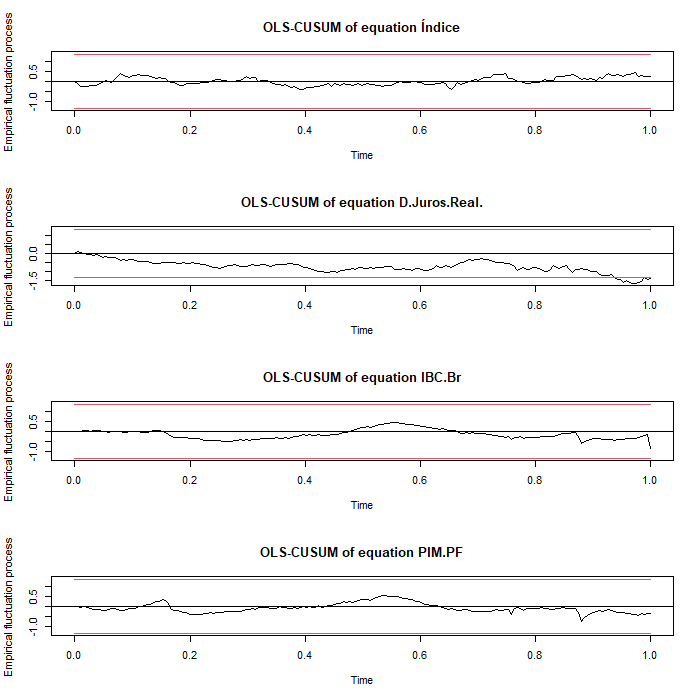
\includegraphics[scale = 0.90]{figuras/ols_cusum_model2.png}
	\fonte{Elaboração do autor.}
\end{figure}

\begin{table}[hbtp]
	\centering
	\caption{Raízes do polinômio característico do VAR($2$)} \label{table:raizes_var_2}
	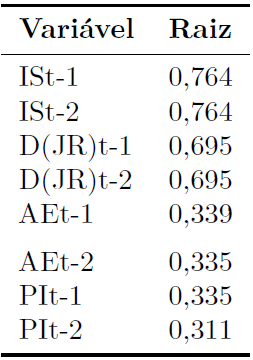
\includegraphics[scale = 0.50]{figuras/raizes_polinomio_caracteristico.PNG}
	\fonte{Elaboração do autor.}
\end{table}

\begin{table}[hbtp]
	\centering
	\caption{Coeficientes da equação do índice de sentimentos do VAR($2$)} \label{table:coef_IS_var_2}
	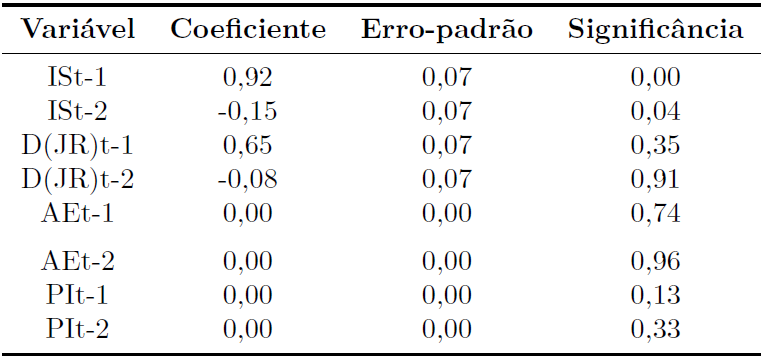
\includegraphics[scale = 0.50]{figuras/coeficientes_IS_var_2.PNG}
	\fonte{Elaboração do autor.}
\end{table}

\begin{table}[hbtp]
	\centering
	\caption{Coeficientes da equação da diferença da taxa de juros real do VAR($2$)} \label{table:coef_JR_var_2}
	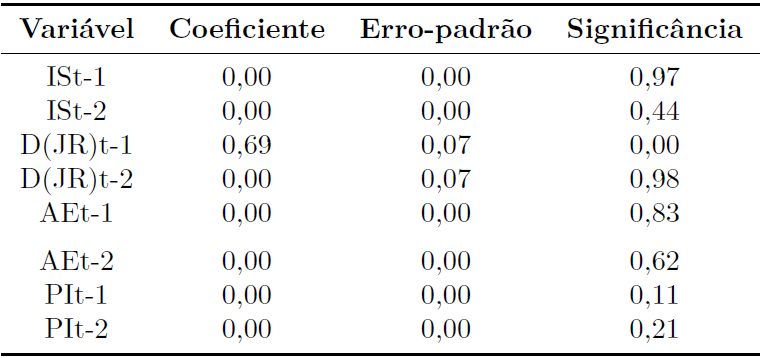
\includegraphics[scale = 0.50]{figuras/coeficientes_JR_var_2.PNG}
	\fonte{Elaboração do autor.}
\end{table}

\begin{table}[hbtp]
	\centering
	\caption{Coeficientes da equação da atividade econômica do VAR($2$)} \label{table:coef_AE_var_2}
	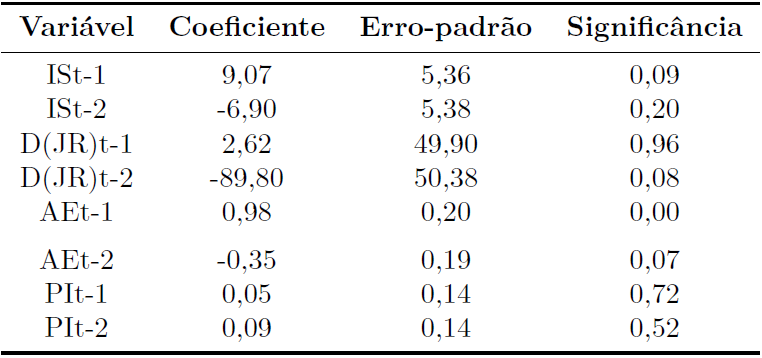
\includegraphics[scale = 0.50]{figuras/coeficientes_AE_var_2.PNG}
	\fonte{Elaboração do autor.}
\end{table}

\begin{table}[hbtp]
	\centering
	\caption{Coeficientes da equação da produção industrial do VAR($2$)} \label{table:coef_PI_var_2}
	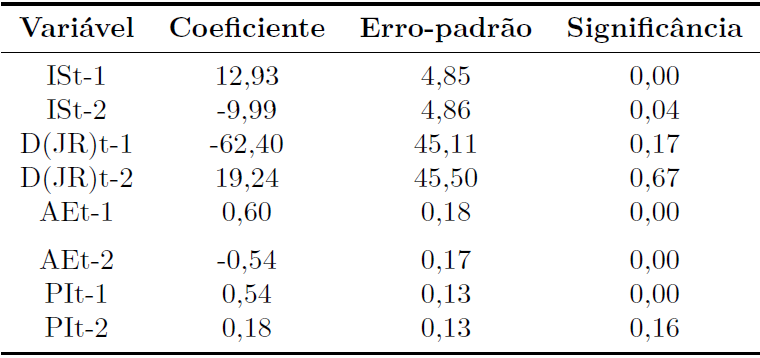
\includegraphics[scale = 0.50]{figuras/coeficientes_PI_var_2.PNG}
	\fonte{Elaboração do autor.}
\end{table}

\chapter{Códigos}

Todos os códigos utilizados no presente trabalho estão disponíveis no repositório online dessa monografia, sendo possível ser acessado por meio deste \href{https://github.com/cairebarletta/tcc}{link}.

\end{apendicesenv}
			    % Elemento Opcional
%% inicia os anexos

\begin{anexosenv}

\chapter{TÍTULO}

\end{anexosenv}
			        % Elemento Opcional
%%índice remissivo (formatado manualmente)

\chapter*{ÍNDICE}
\addcontentsline{toc}{chapter}{ÍNDICE}

{ \setlength{\parindent}{0pt}  % ambiente sem indentação
	
Andesito, 22, 50, 73

Argila, 52, 75, 121

Basalto, 25, 230, 235

} % fim ambiente sem indentação		% Elemento Opcional

\end{document}